\documentclass[letterpaper,9pt]{article}

\usepackage{threeparttable}
\usepackage{geometry}
\geometry{letterpaper,tmargin=1.0in,bmargin=1.0in,lmargin=1.0in,rmargin=1.0in}
\usepackage[format=hang,font=normalsize,labelfont=bf]{caption}
\usepackage{amsmath}
\usepackage{multirow}
\usepackage{array}
\usepackage{delarray}
\usepackage{amssymb}
\usepackage{amsthm}
\usepackage{lscape}
\usepackage{natbib}
\usepackage{setspace}
\usepackage{float,color}
\usepackage[pdftex]{graphicx}
\usepackage{subfigure} % Allows multiple subfigures in one figure 
\usepackage{caption}
\usepackage{subcaption}
\usepackage{listings}
\lstset{basicstyle=\footnotesize\ttfamily, language=Python, showstringspaces=false}

\lstset{frame=single,
  language=Python,
  showstringspaces=false,
  columns=flexible,
  basicstyle={\small\ttfamily},
  numbers=none,
  breaklines=true,
  breakatwhitespace=true
  tabsize=3
}

\usepackage{pdfsync}
\usepackage{booktabs}
\usepackage{verbatim}
\usepackage{placeins}
\usepackage{geometry}
\usepackage{pdflscape}
\synctex=1
\usepackage{hyperref}
\hypersetup{colorlinks,linkcolor=black,urlcolor=blue,citecolor=black}
\usepackage{bm}


\theoremstyle{definition}
\newtheorem{theorem}{Theorem}
\newtheorem{acknowledgement}[theorem]{Acknowledgement}
\newtheorem{algorithm}[theorem]{Algorithm}
\newtheorem{axiom}[theorem]{Axiom}
\newtheorem{case}[theorem]{Case}
\newtheorem{claim}[theorem]{Claim}
\newtheorem{conclusion}[theorem]{Conclusion}
\newtheorem{condition}[theorem]{Condition}
\newtheorem{conjecture}[theorem]{Conjecture}
\newtheorem{corollary}[theorem]{Corollary}
\newtheorem{criterion}[theorem]{Criterion}
\newtheorem{definition}{Definition}  % Number definitions on their own
\newtheorem{derivation}{Derivation}  % Number derivations on their own
\newtheorem{example}[theorem]{Example}
\newtheorem{exercise}[theorem]{Exercise}
\newtheorem{lemma}[theorem]{Lemma}
\newtheorem{notation}[theorem]{Notation}
\newtheorem{problem}[theorem]{Problem}
\newtheorem{proposition}{Proposition}  % Number propositions on their own
\newtheorem*{proposition*}{Proposition}  % Non-numbered proposition
\newtheorem{remark}[theorem]{Remark}
\newtheorem{solution}[theorem]{Solution}
\newtheorem{summary}[theorem]{Summary}
\bibliographystyle{aer}
\newcommand\ve{\varepsilon}
%\renewcommand\theenumi{\roman{enumi}}
\newcommand\norm[1]{\left\lVert#1\right\rVert}


\title{What can LLMs tell us about the ETI?}
\author{
  \href{http://jasondebacker.com/}{Jason DeBacker}\thanks{University of South Carolina, Darla Moore School of Business, Department of Economics, \href{mailto:jason.debacker@moore.sc.edu}{jason.debacker@moore.sc.edu}.}
  \and
  {Max Ghenis}\thanks{\href{https://policyengine.org/}{PolicyEngine}, \href{mailto:max@policyengine.org}{max@policyengine.org}.}
  \and
  {Roxana Gonzalez}\thanks{University of South Carolina, Darla Moore School of Business, Department of Economics, \href{mailto:roxanag@email.sc.edu}{roxanag@email.sc.edu}. Code and data to replicate the results are available on GitHub at \url{https://github.com/MaxGhenis/llm-eti}.}
}
\date{\today}


\begin{document}

\begin{titlepage}
\maketitle
\vspace{-2mm}
\begin{abstract}
\small{This paper investigates the capacity of large language models (LLMs) to approximate the elasticity of taxable income (ETI), a central parameter in public finance. We use LLMs to simulate a seminal study using observational data \citep{GruberSaez2002} and conduct simulations based on a recent controlled experiment \citep{PKNF2024} to evaluate how five popular LLMs respond to tax schedule changes. Our results show that LLMs reproduce key behavioral patterns observed in human studies, though often with heightened responsiveness, suggesting limited recognition of real-world frictions. This study provide an approach that can be used to benchmark LLM responses to questions of the behavioral responses of taxation. In the future, LLMs may have potential as low-cost, flexible complements to traditional methods for analyzing taxpayer behavior and policy design, although further validation across models and contexts is needed.
}

\vspace{10mm}

\noindent\textit{keywords:}\: AI, elasticity of taxable income

\vspace{10mm}

\noindent\textit{JEL classification:} H21, H31 


\end{abstract}
\thispagestyle{empty}
\end{titlepage}


\begin{spacing}{1.5}

\pagenumbering{arabic}

\section{Introduction}
Large language models (LLMs) have been found to replicate human behavior in economic contexts. \cite{horton2023large} show that LLMs endowed with preferences and information reproduce the qualitative results of several classic behavioral experiments. \cite{BIN2023} estimate demand functions implied from an LLM and find that they match very closely those estimated from human preferences. \cite{BrookinsDeBacker2024}, \cite{mei2024turing}, and \cite{akata2025playing} show that LLMs exhibit human-like cooperation in strategic games.

A related finding is that LLMs tend to behave more like frictionless optimizing agents than human subjects do, whose observed responses are attenuated by adjustment costs, inattention, and other optimization frictions. \cite{chen2023emergence} find that GPT's budgetary decisions are largely consistent with utility maximization under revealed preference theory, scoring higher on rationality measures than human subjects. \cite{AHGW2024} and \cite{cui2025large} use LLMs to replicate a range of social science experiments with human subjects, finding that LLM responses reproduce the direction and significance of most human treatment effects, though with a tendency to overstate effect sizes.

This paper extends the research on LLM responses in an economic context to explore an important parameter in public finance economics: the elasticity of taxable income (ETI).  If LLMs are insightful regarding the ETI, there is potential for new research methods and questions and for the application of LLMs to tax policy and administration. LLMs may allow one to explore heterogeneity one can't identify in observational data. For example, while religion is not measured in administrative tax data, there may be interesting differences in the elasticity of taxable income through differences in charitable giving across religiosity. LLMs also allow researchers to simulate tax policies that have not existed and approximate human responses. Even when laboratory or field experiments can be employed to measure taxpayer behavior, LLMs are orders of magnitude cheaper and may act as a substitute (or complement) to such experiments.

Furthermore, if LLMs prove insightful in this context, tax practitioners can use these to quickly explore how taxpayers might respond to changes in tax law or regulation, or to simulate hypothetical scenarios. Practitioners may also use LLMs to decompose different margins of responses (e.g., reporting versus real responses) that may not be directly observable in the data.

We take two approaches to elicit ETI estimates from five different LLMs. First,  we use LLMs to simulate taxpayer responses in the spirit of the observational data used in \cite{GruberSaez2002}, a seminal empirical study of the ETI. Next, we replicate the controlled lab experiment of \cite{PKNF2024} in which subjects decide on labor supply under changing tax schedules, but prompt LLMs rather than humans. 

Our findings suggest that LLMs are broadly consistent with empirical estimates of the ETI. In the observational setting, the overall ETI estimate across models of 0.378 is consistent with the \cite{GruberSaez2002} estimate of 0.4. In the experimental setting, we find the behavior of LLMs to be much more rational than human subjects in their responses to changes in marginal tax rates. When faced with a tax notch, the LLMs never locate in the dominated region, which is not the case for the human participants. This suggests that LLMs may not take into consideration certain frictions or be subject to the cognitive limitations faced by human participants.

The remainder of this paper is organized as follows. Section \ref{sec:Obs} describes the use of LLMs in simulating the study  of \cite{GruberSaez2002}. Section \ref{sec:Lab} presents the replication of \cite{PKNF2024}. Section \ref{sec:Conclude} offers concluding thoughts.

\section{An Observational-Style Simulation}
\label{sec:Obs}

We simulated an observational data study using LLMs, following a seminal empirical study of the ETI, \cite{GruberSaez2002}. The authors use a panel data approach and variation in marginal tax rates over time and across states through tax reforms.  Because marginal tax rates, being a function of income, are endogenous, they instrument for marginal tax rates with prior year income.

Replicating a study using observational data through an LLM is less straightforward than a lab experiment as in Section \ref{sec:Lab}. Thus one should not interpret our results as a direct replication of the methods in \cite{GruberSaez2002} and thus our estimand is not identical. Rather we want to try to mimic the general identification strategy used in the observational study. We do this by prompting the LLM with taxpayer scenarios with random variation in income and marginal tax rates.  We further specify that broad income before behavioral adjustments will be similar to last year’s income to capture the instrumental approach of \cite{GruberSaez2002}. The exact prompt takes the following form: \\


  \framebox{%
   \begin{minipage}{15cm}
   \vspace{0.4cm}
    \begin{quote}
        You are a taxpayer with the following tax profile:\\
            - Last year, your broad income was [\$X]\\
            - Last year, your taxable income was [\$Y]\\
            - Last year, your marginal tax rate was [$r$ \%]\\
            
        Due to a change in tax law, your marginal tax rate this year will be $r'$ \%.
        Your broad income before any adjustments or changes in behavior would be
        approximately the same as last year.

        Given this change in tax rates, you may adjust your behavior -- for example,
        how much you work, your charitable contributions, retirement savings, or the
        timing of income realizations like capital gains.
        \vspace{0.4cm}
    \end{quote}
   \end{minipage}
  } \vspace{0.8cm}
  
Broad and taxable income are drawn from records in PolicyEngine's Enhanced CPS file, which fuses the Census Current Population Survey with the Internal Revenue Service Public Use File.\footnote{\url{https://policyengine.github.io/policyengine-us-data/}}. This ensures an randomized sample of taxpayers that are representative of the US taxpaying population. Last year's marginal tax rates are computed through PolicyEngine for each record and so are consistent with the taxable and broad income measures for that record. The current year marginal tax rates are last year's marginal rate times a random shock. The random component is drawn from a log-normal distribution with mean one and a standard deviation of 0.025.

In repeated calls to the LLMs' APIs, we collect 2,000 responses from each of five LLMs: GPT-4o, GPT-4o-mini, Claude Haiku 4.5, DeepSeek V3, and Gemma 4.  The total number of observations from these simulations is 9,649 after excluding non-numeric or otherwise unusable responses.

We compute the taxpayer's elasticities of taxable (broad) income for each simulation by finding the percentage change in reported taxable (broad) income for the percentage change in the marginal tax rates they face.  Table \ref{tab:obs_summ_stats} presents the mean and median ETI from each LLM.  With GPT-4o-mini, DeepSeek V3, and Gemma 4, the mean ETIs (0.462, 0.428, and 0.593), are close to those found by \cite{GruberSaez2002}, 0.40. Models GPT-4o and Claude Haiku 4.5 deviate substantially from this pattern, with means of -0.046 and 0.849, respectively.

Mean values, however, mask a great deal of heterogeneity. Across all models but Claude Haiku 4.5, median ETIs are zero and 22.1-30\% of a model's responses report current-year taxable income equal to the prior-year value assigned to them. With Claude Haiku 4.5, we see much more variation in the reported taxable income, with just 10\% reporting the value they had in the previous year. The overall mean ETI across all models is 0.458 with a median ETI of 0.0.
\vspace{0.6cm}

\begin{table}[!htbp] \centering
  \caption{Model Comparison: Summary Statistics; Gruber \& Saez 2002, Table 2}
  \label{tab:obs_summ_stats}
  \begin{tabular}{lcccccc}
  \toprule
  & GPT-4o & \shortstack{GPT-4o \\ mini} & \shortstack{Claude \\ Haiku 4.5} & \shortstack{DeepSeek \\ V3} & Gemma 4 & \shortstack{All \\ Models} \\
  \midrule
  Mean ETI & -0.046 & 0.462 & 0.849 & 0.428 & 0.593 & 0.458 \\
  Median ETI & 0.000 & 0.000 & 0.653 & 0.000 & 0.000 & 0.000 \\
  \% Same Income & 27.8\% & 23.7\% & 10.0\% & 22.1\% & 30.0\% & 22.7\% \\
  \midrule
  Observations & 2,000 & 1,997 & 2,000 & 1,678 & 1,974 & 9,649 \\
  \bottomrule
  \end{tabular}
  \begin{flushleft}\footnotesize
  Table reports the analogous statistics to row 2 of Table 2 in \cite{GruberSaez2002}, broken up by LLM. All dollar values are expressed in 2026 dollars.\\
  \end{flushleft}
\end{table}

\subsection{Baseline ETI estimates}

We estimate the elasticity of both broad and taxable income in the classic framework of regressing log income on the net-of-tax rate as done in \cite{GruberSaez2002}.  In our case, we randomized the marginal tax rates in the prompts to our LLM and therefore use ordinary least squares regressions on the LLM output, rather than an instrumental variables approach.  Following \cite{GruberSaez2002}, we control for base income with a spline in these regressions.  The regression results are reported in Tables \ref{tab:obs_regs_broad} (broad income) and \ref{tab:obs_regs_taxable} (taxable income).

\begin{table}[!htbp] \centering
  \caption{Model Comparison: Elasticity Results (Broad Income); Gruber \& Saez 2002, Table 4}
  \label{tab:obs_regs_broad}
  \begin{tabular}{lcccccc}
  \toprule
  & GPT-4o & \shortstack{GPT-4o \\ mini} & \shortstack{Claude \\ Haiku 4.5} & \shortstack{DeepSeek \\ V3} & Gemma 4 & \shortstack{All \\ Models} \\
  \midrule
  Constant & $0.000$ & $-0.001^{***}$ & $-0.003^{***}$ & $-0.000^{*}$ & $-0.001^{**}$ & $-0.001^{***}$ \\
  & (0.000) & (0.000) & (0.000) & (0.000) & (0.000) & (0.000) \\
  Net-of-tax elasticity & $0.017^{***}$ & $0.048^{***}$ & $0.440^{***}$ & $0.000$ & $0.012^{*}$ & $0.107^{***}$ \\
  & (0.004) & (0.009) & (0.015) & (0.000) & (0.006) & (0.005) \\
  Base income spline 1 & $0.001^{*}$ & $0.001$ & $-0.003$ & $0.000$ & $-0.000$ & $-0.000$ \\
  & (0.001) & (0.001) & (0.002) & (0.000) & (0.000) & (0.001) \\
  Base income spline 2 & $-0.000$ & $0.000$ & $0.001^{**}$ & $-0.000$ & $0.001^{**}$ & $0.000^{*}$ \\
  & (0.000) & (0.001) & (0.001) & (0.000) & (0.000) & (0.000) \\
  Base income spline 3 & $-0.000^{*}$ & $-0.001$ & $0.001^{**}$ & $-0.000$ & $-0.000$ & $0.000$ \\
  & (0.000) & (0.000) & (0.001) & (0.000) & (0.000) & (0.000) \\
  Base income spline 4 & $-0.000$ & $0.001$ & $0.002^{**}$ & $0.000$ & $0.000^{*}$ & $0.001^{**}$ \\
  & (0.000) & (0.001) & (0.001) & (0.000) & (0.000) & (0.000) \\
  Base income spline 5 & $-0.000$ & $-0.002$ & $-0.005^{**}$ & $0.000$ & $-0.001^{**}$ & $-0.002^{**}$ \\
  & (0.000) & (0.002) & (0.002) & (0.000) & (0.001) & (0.001) \\
  \midrule
  $R^2$ & 0.036 & 0.032 & 0.352 & 0.003 & 0.007 & 0.079 \\
  \midrule
  N & 2,000 & 1,982 & 2,000 & 1,678 & 1,973 & 9,633 \\
  \bottomrule
  \end{tabular}
  \begin{flushleft}\footnotesize
  Table reports the analogous estimates to column 5 from Table 4 in \cite{GruberSaez2002}, broken up by LLM. Heteroskedasticity-robust SEs in parentheses. Specifications include a natural cubic spline (df\,$=$5) in log base-year income; its five basis-term coefficients are reported as ``Base income spline 1--5''.\\
  $^{*}p<0.1$, $^{**}p<0.05$, $^{***}p<0.01$
  \end{flushleft}
\end{table}
\begin{table}[!htbp] \centering
  \caption{Model Comparison: Elasticity Results (Taxable Income); Gruber \& Saez 2002, Table 4}
  \label{tab:obs_regs_taxable}
  \begin{tabular}{lcccccc}
  \toprule
  & GPT-4o & \shortstack{GPT-4o \\ mini} & \shortstack{Claude \\ Haiku 4.5} & \shortstack{DeepSeek \\ V3} & Gemma 4 & \shortstack{All \\ Models} \\
  \midrule
  Constant & $-0.002^{*}$ & $-0.003^{***}$ & $-0.013^{***}$ & $-0.004^{***}$ & $0.013$ & $-0.003$ \\
  & (0.001) & (0.001) & (0.005) & (0.001) & (0.012) & (0.003) \\
  Net-of-tax elasticity & $0.031^{**}$ & $0.361^{***}$ & $0.792^{***}$ & $0.406^{***}$ & $0.289^{***}$ & $0.378^{***}$ \\
  & (0.015) & (0.033) & (0.035) & (0.027) & (0.107) & (0.026) \\
  Base income spline 1 & $-0.009$ & $-0.003$ & $-0.061^{**}$ & $-0.005$ & $0.072$ & $-0.005$ \\
  & (0.007) & (0.005) & (0.025) & (0.005) & (0.063) & (0.013) \\
  Base income spline 2 & $0.002$ & $-0.001$ & $0.009^{*}$ & $0.001$ & $-0.015$ & $-0.000$ \\
  & (0.001) & (0.002) & (0.005) & (0.001) & (0.012) & (0.003) \\
  Base income spline 3 & $0.002$ & $-0.002$ & $0.013^{**}$ & $0.002^{*}$ & $-0.016$ & $0.000$ \\
  & (0.001) & (0.001) & (0.005) & (0.001) & (0.013) & (0.003) \\
  Base income spline 4 & $0.001$ & $-0.001$ & $0.009^{*}$ & $0.001$ & $-0.012$ & $0.000$ \\
  & (0.001) & (0.001) & (0.005) & (0.001) & (0.012) & (0.003) \\
  Base income spline 5 & $0.002$ & $0.003$ & $0.017^{***}$ & $-0.003$ & $-0.016$ & $0.002$ \\
  & (0.002) & (0.003) & (0.006) & (0.003) & (0.014) & (0.003) \\
  \midrule
  $R^2$ & 0.015 & 0.072 & 0.262 & 0.229 & 0.019 & 0.045 \\
  \midrule
  N & 1,998 & 1,928 & 1,999 & 1,678 & 1,950 & 9,553 \\
  \bottomrule
  \end{tabular}
  \begin{flushleft}\footnotesize
  Table reports the analogous estimates to column 6 from Table 4 in \cite{GruberSaez2002}, broken up by LLM. Heteroskedasticity-robust SEs in parentheses. Specifications include a natural cubic spline (df\,$=$5) in log base-year income; its five basis-term coefficients are reported as ``Base income spline 1--5''.\\
  $^{*}p<0.1$, $^{**}p<0.05$, $^{***}p<0.01$
  \end{flushleft}
\end{table}

Consistent with the findings of \cite{GruberSaez2002}, we find the elasticity of taxable income to be larger than the elasticity of broad income.  Across all models, the elasticity of broad income with respect to the net-of-tax rate is 0.107. In their specification with income spline controls, \cite{GruberSaez2002} find this elasticity to be 0.120. As with the summary statistics above, there is considerable variation across models with Claude being the most responsive (elasticity of 0.44) and DeepSeek simulations not showing any change in broad income, resulting in an elasticity of 0. 

The elasticity of taxable income across all models and simulations is 0.378, which again is close to the estimate from \cite{GruberSaez2002} of 0.400.  The GPT-4o-mini and DeepSeek models elicit elasticities in this range (estimates of 0.361 and 0.406, respectively).  Claude again is the most responsive (ETI of 0.792), while GPT-4o is the least responsive (ETI of 0.031).

\subsection{Variation in the ETI across income groups}

An important result of \cite{GruberSaez2002} is that the elasticity of taxable income varies across the income distribution with higher income taxpayers having larger elasticities. To test this, we create three income groups with similar income ranges to those used in \cite{GruberSaez2002} using the Consumer Price Index to inflate their income ranges to 2026 dollars.  We then regress log income on the net-of-tax rate, allowing for separate coefficients for each of the three bins.  Table \ref{tab:obs_regs_income} contains the coefficient estimates from the net-of-tax rate term, the standard error and the number of observations in each income group. All LLM model simulations are used in these regressions. The key finding is that the elasticities of income with the net-of-tax rate do not vary across income groups.  This contrasts with the findings of \cite{GruberSaez2002} and suggests that LLMs are missing some of the context that humans have in their responses such as frictions one might face when trying to adjust earnings.

\begin{table}[!htbp] \centering
  \caption{Elasticity Results by Income Group, \textit{All Models} (CPI-adjusted to 2026\$; Gruber \& Saez 2002, Table 9)}
  \label{tab:obs_regs_income}
  \begin{tabular}{lccc}
  \toprule
  Income range & \shortstack{Broad \\ income (1)} & \shortstack{Taxable \\ income (2)} & \shortstack{Taxable inc. \\ (tax. cuts) (3)} \\
  \midrule
  \$24K--\$118K (\$24K--\$75K) & $0.113^{***}$ & $0.341^{***}$ & $0.339^{***}$ \\
  & (0.006) & (0.017) & (0.020) \\
  N. Obs & 6,195 & 6,161 & 3,803 \\[10pt]
  \$118K--\$235K (\$75K--\$176K) & $0.104^{***}$ & $0.290^{***}$ & $0.307^{***}$ \\
  & (0.010) & (0.018) & (0.018) \\ 
  N. Obs & 2,026 & 2,022 & 2,307 \\[10pt]
  \$235K+ (\$176K+) & $0.090^{***}$ & $0.244^{***}$ & $0.246^{***}$ \\
  & (0.011) & (0.023) & (0.021) \\ 
  N. Obs & 836 & 836 & 978 \\[2pt]
  \bottomrule
  \end{tabular}
  \begin{flushleft}\footnotesize
  Each cell: income-weighted OLS elasticity of income with respect to the net-of-tax rate, estimated within the base-year income group. Heteroskedasticity-robust SEs in parentheses. Columns (1)--(2) split the sample by base-year broad income; column (3) by base-year taxable income. Groups control for base-year income via a natural cubic spline (df\,$=$5), or a single linear term when N\,$<$150. OLS rather than 2SLS because the net-of-tax rate change is imposed by the simulation. Income ranges are GS's 1992-dollar cutoffs inflated to 2026 dollars with CPI-U (factor 2.35); the 2026 CPI value is an estimate.\\
  $^{*}p<0.1$, $^{**}p<0.05$, $^{***}p<0.01$
  \end{flushleft}
\end{table}
\vspace{0.6cm}

\subsection{Variation in the ETI by marginal tax rate change}

Figure ~\ref{fig:eti_by_mtr_model} displays taxable income elasticity estimates by size of the marginal tax rate change, broken out by model. Three models, GPT-4o-mini, Claude Haiku 4.5, and DeepSeek V3, yield elasticities that are concentrated around and just above 0.40. GPT-4o, by contrast, concentrates at zero with almost no dispersion. No observations are seen at a rate change of zero as all prompts included a nonzero rate change by construction. Notably, while the dispersion of the elasticities increases with the absolute value of the change in marginal tax rates, the mean value of the elasticity does not.

    \begin{figure}
    \centering
    \caption{Elasticity of Taxable Income by Marginal Tax Rate Change}
    \label{fig:eti_by_mtr_model}
    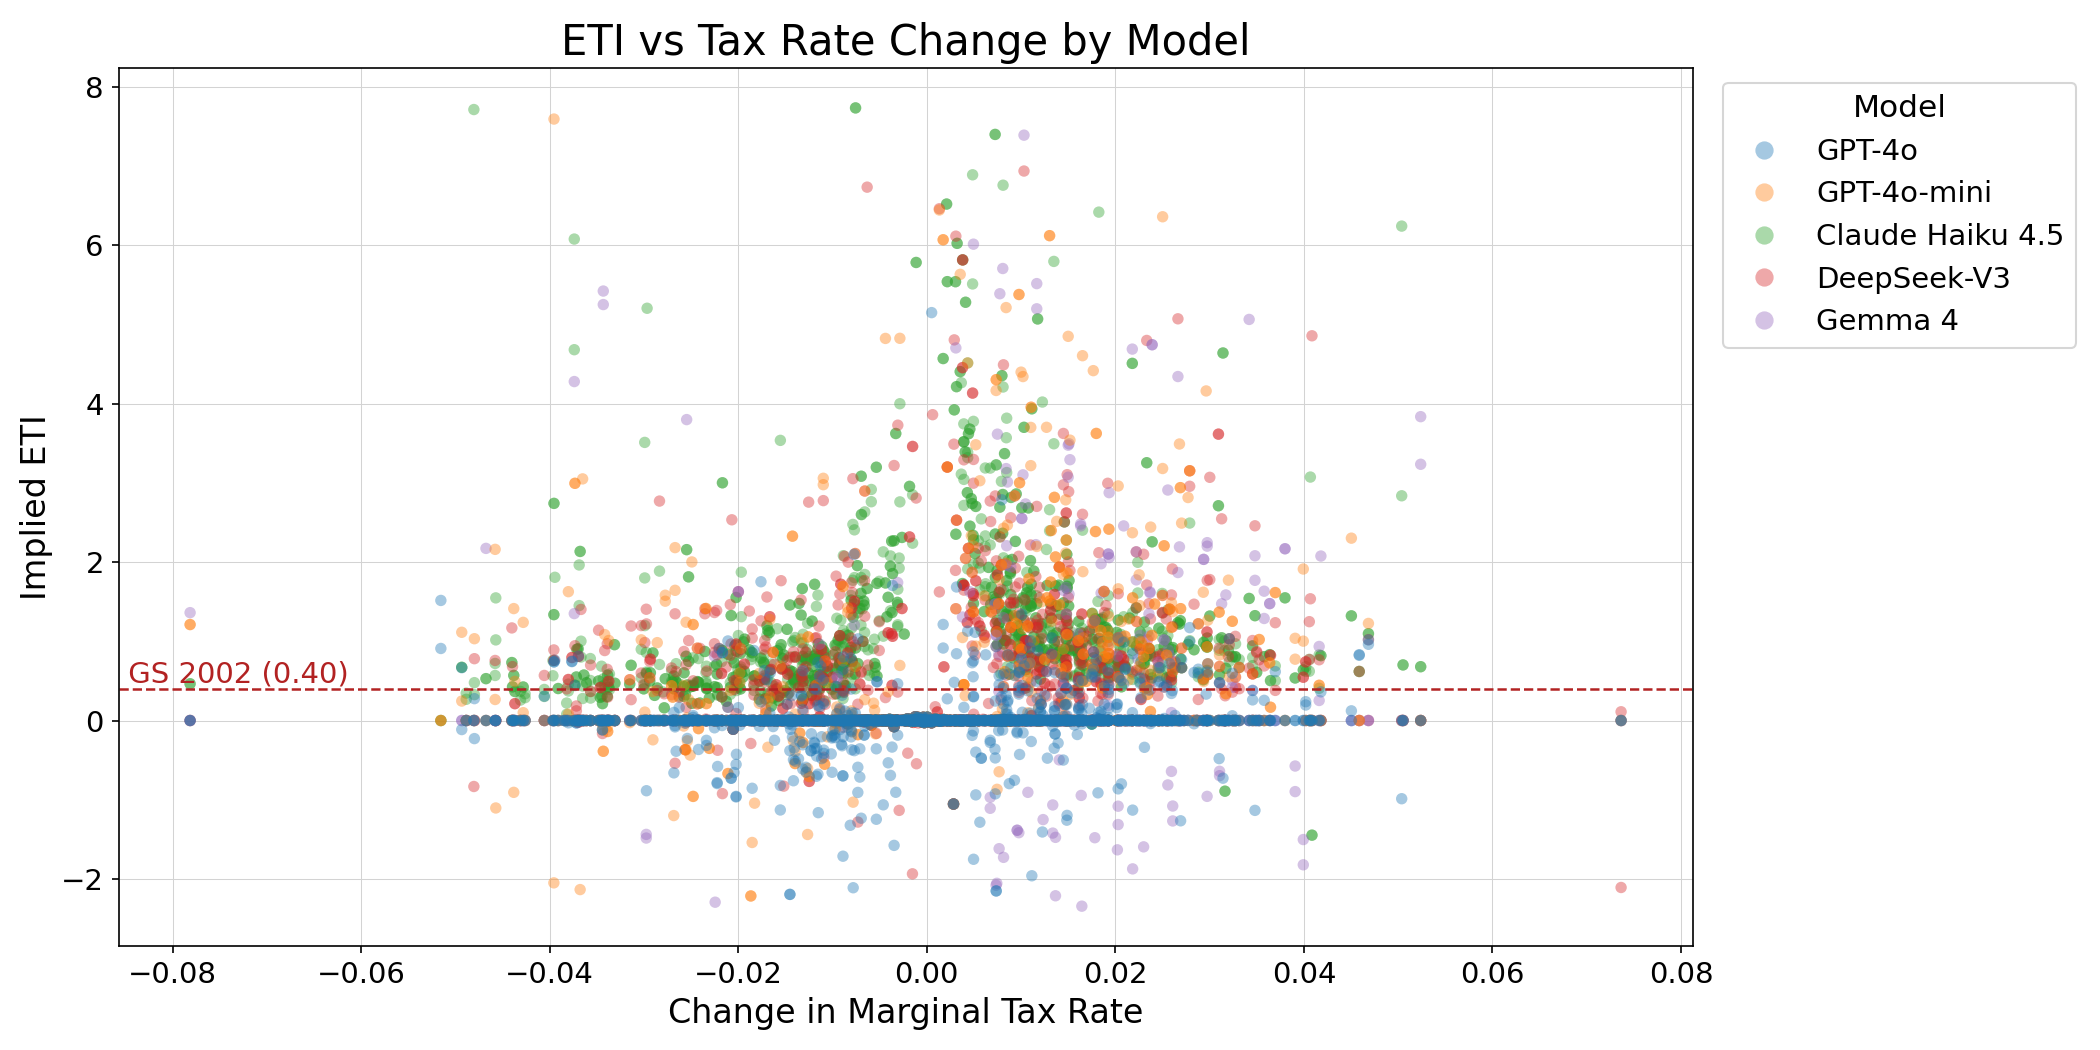
\includegraphics[width=0.9\textwidth]{images_tables/eti_by_mtr_model.png} \\
    \small{Figure notes: ETI estimates by size of marginal tax rate change, broken out by model. Red dashed horizontal line represents the headline ETI estimate of 0.40 from \cite{GruberSaez2002}.}
    \end{figure}

\section{Replicating a Lab Experiment}
\label{sec:Lab}

We now turn to replicating an experimental design. \cite{PKNF2024} (PKNF) provide an experimental framework to measure labor supply responses to changes in effective and marginal tax rates. In their study, subjects play a 16-round game. In each round, players are given a tax schedule and a randomly drawn labor endowment (from 14 to 30 units) and then decide how much to work. After eight rounds, there is a reform to the tax system, which persists for the final eight rounds.  There are three different tax schedules considered: a flat marginal tax rate of 25\%, a flat marginal tax rate of 50\%, and a system with a notch where the average (and marginal) tax rate is 25\% up to a labor supply of 20 and then the average and marginal rates jump up to 50\%.  The reform either removes or adds a notch to the tax system. Subjects have to perform work (typing characters) based on their responses in a randomly selected round.

We use the same economic context as \cite{PKNF2024} with the same tax schedules and 16 rounds of play. We provide the same instructions to the LLMs that they provided to their human participants. Because we use LLMs, we make one deviation: we do not require them to perform the work from a randomly selected round (recall, the human subjects typed characters). While LLMs lack authentic preferences between consumption and leisure and may therefore over-respond to tax incentives, the absence of an actual labor task dampens measured labor supply responses relative to humans. The net bias to estimated ETI remains ambiguous.

\subsection{Labor Supply Responses to Notches}
Results from \cite{PKNF2024} and from simulations using five LLMs are presented side-by-side in Figure \ref{fig:LabSupply}.  In the \cite{PKNF2024} study, 78-88\% of player-rounds show a labor supply less than 20 units (out of a maximum of 30) when there is a notch in the tax system (what \cite{PKNF2024} call a progressive tax schedule). When there is a flat tax (either at a 25\% or 50\% rate) 46 to 54\% of player-rounds yield a labor supply less than 20 units.  In the LLM responses, the percentage of player-rounds with a labor supply below 20 is higher than in the study using human subjects; it is close to 100\% in all models when the progressive tax system is simulated. This is a difference of about 20 percentage points, on average, indicating that LLMs find the notch much more salient than human subjects.  The exception is GPT-4o-mini: around 42\% of simulated responses have labor supply under 20 units regardless of the tax system. Under the flat taxes, the LLM responses are more similar to those from human subjects with 36 to 46\% of responses yielding a labor supply less than 20 units, compared to rates of 46 to 54\% for the human subjects. Results are quite similar across models, other than GPT-4o-mini. Because of this, our next two figures will refer to results only for the GPT-4o model to ease exposition.\footnote{Results for other models are presented in the appendix.}

    % \begin{table}
    % \centering
    % \caption{Fraction of subjects with labor supply $<$ 20:}
    % \input{images_tables/table5_both}
    % \label{tab:LabSupply}
    % \end{table}

    \begin{figure}[h]
        \centering
        \label{fig:lab_supply20_round}
         \subfigure[Pre-Reform]{
       	 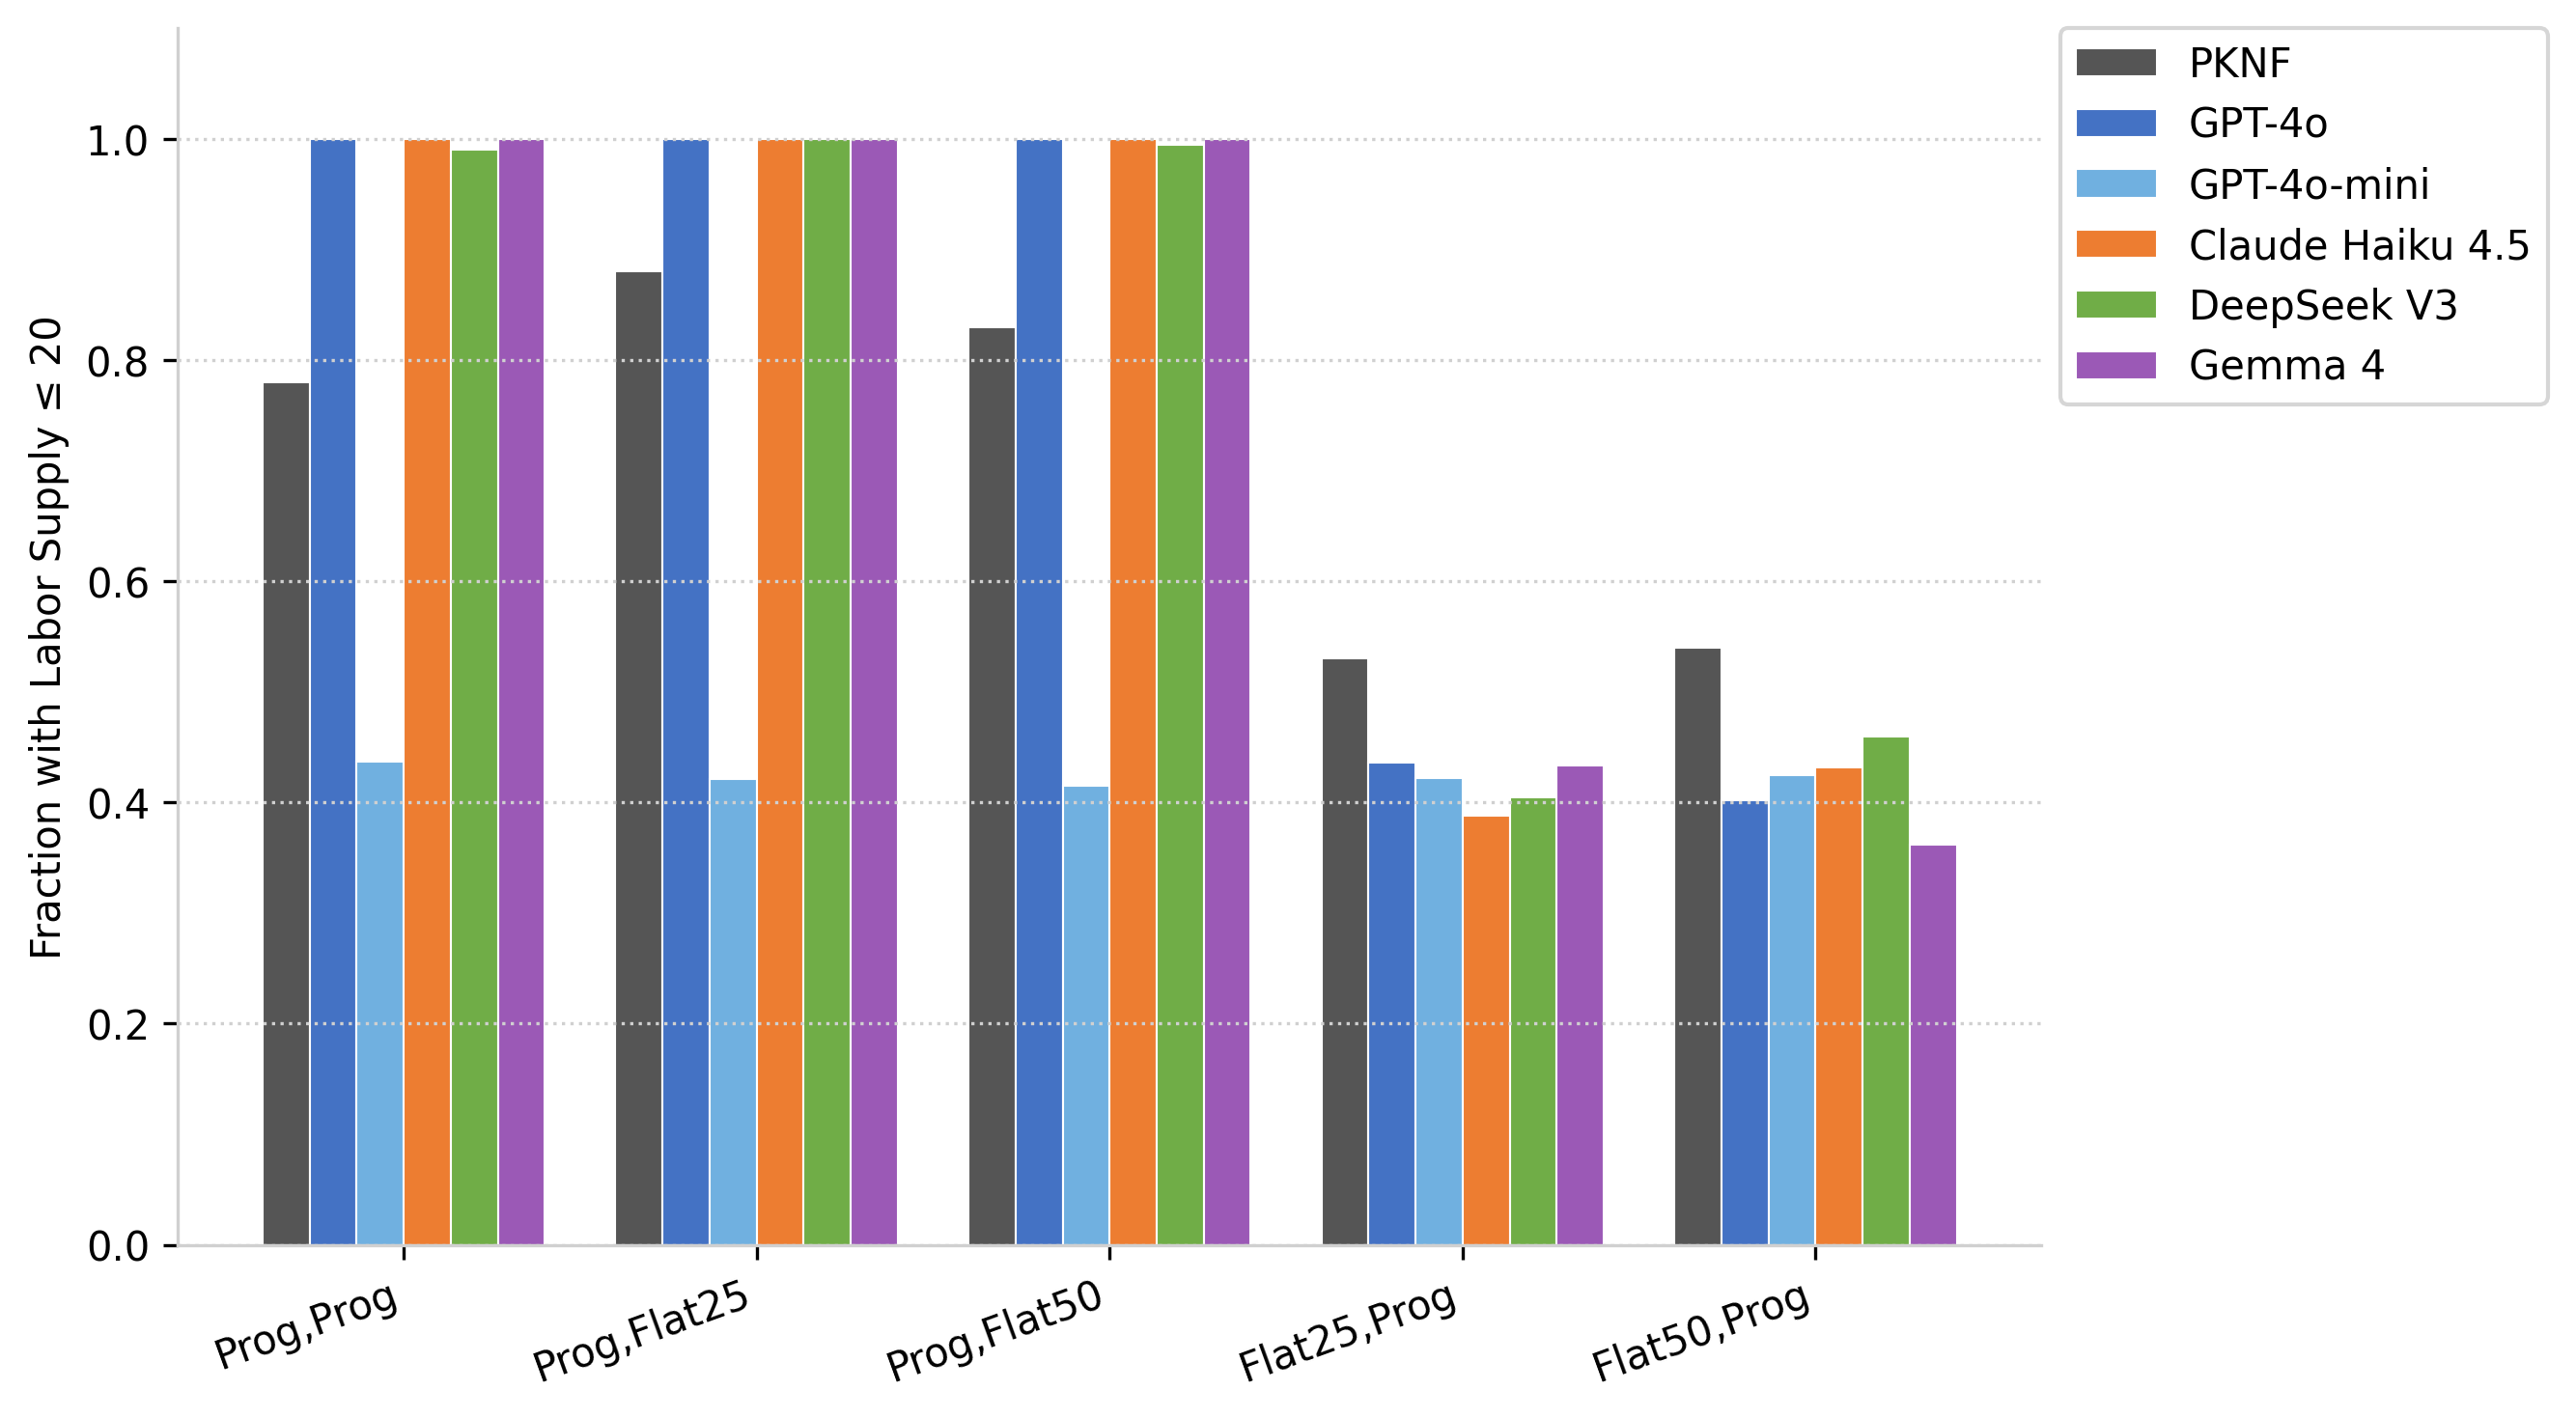
\includegraphics[width=0.55\textwidth]{images_tables/pknf_all_models_25pct_50pct_table5_bar_pre.png}
    	}
        \subfigure[Post-Reform]{
       	 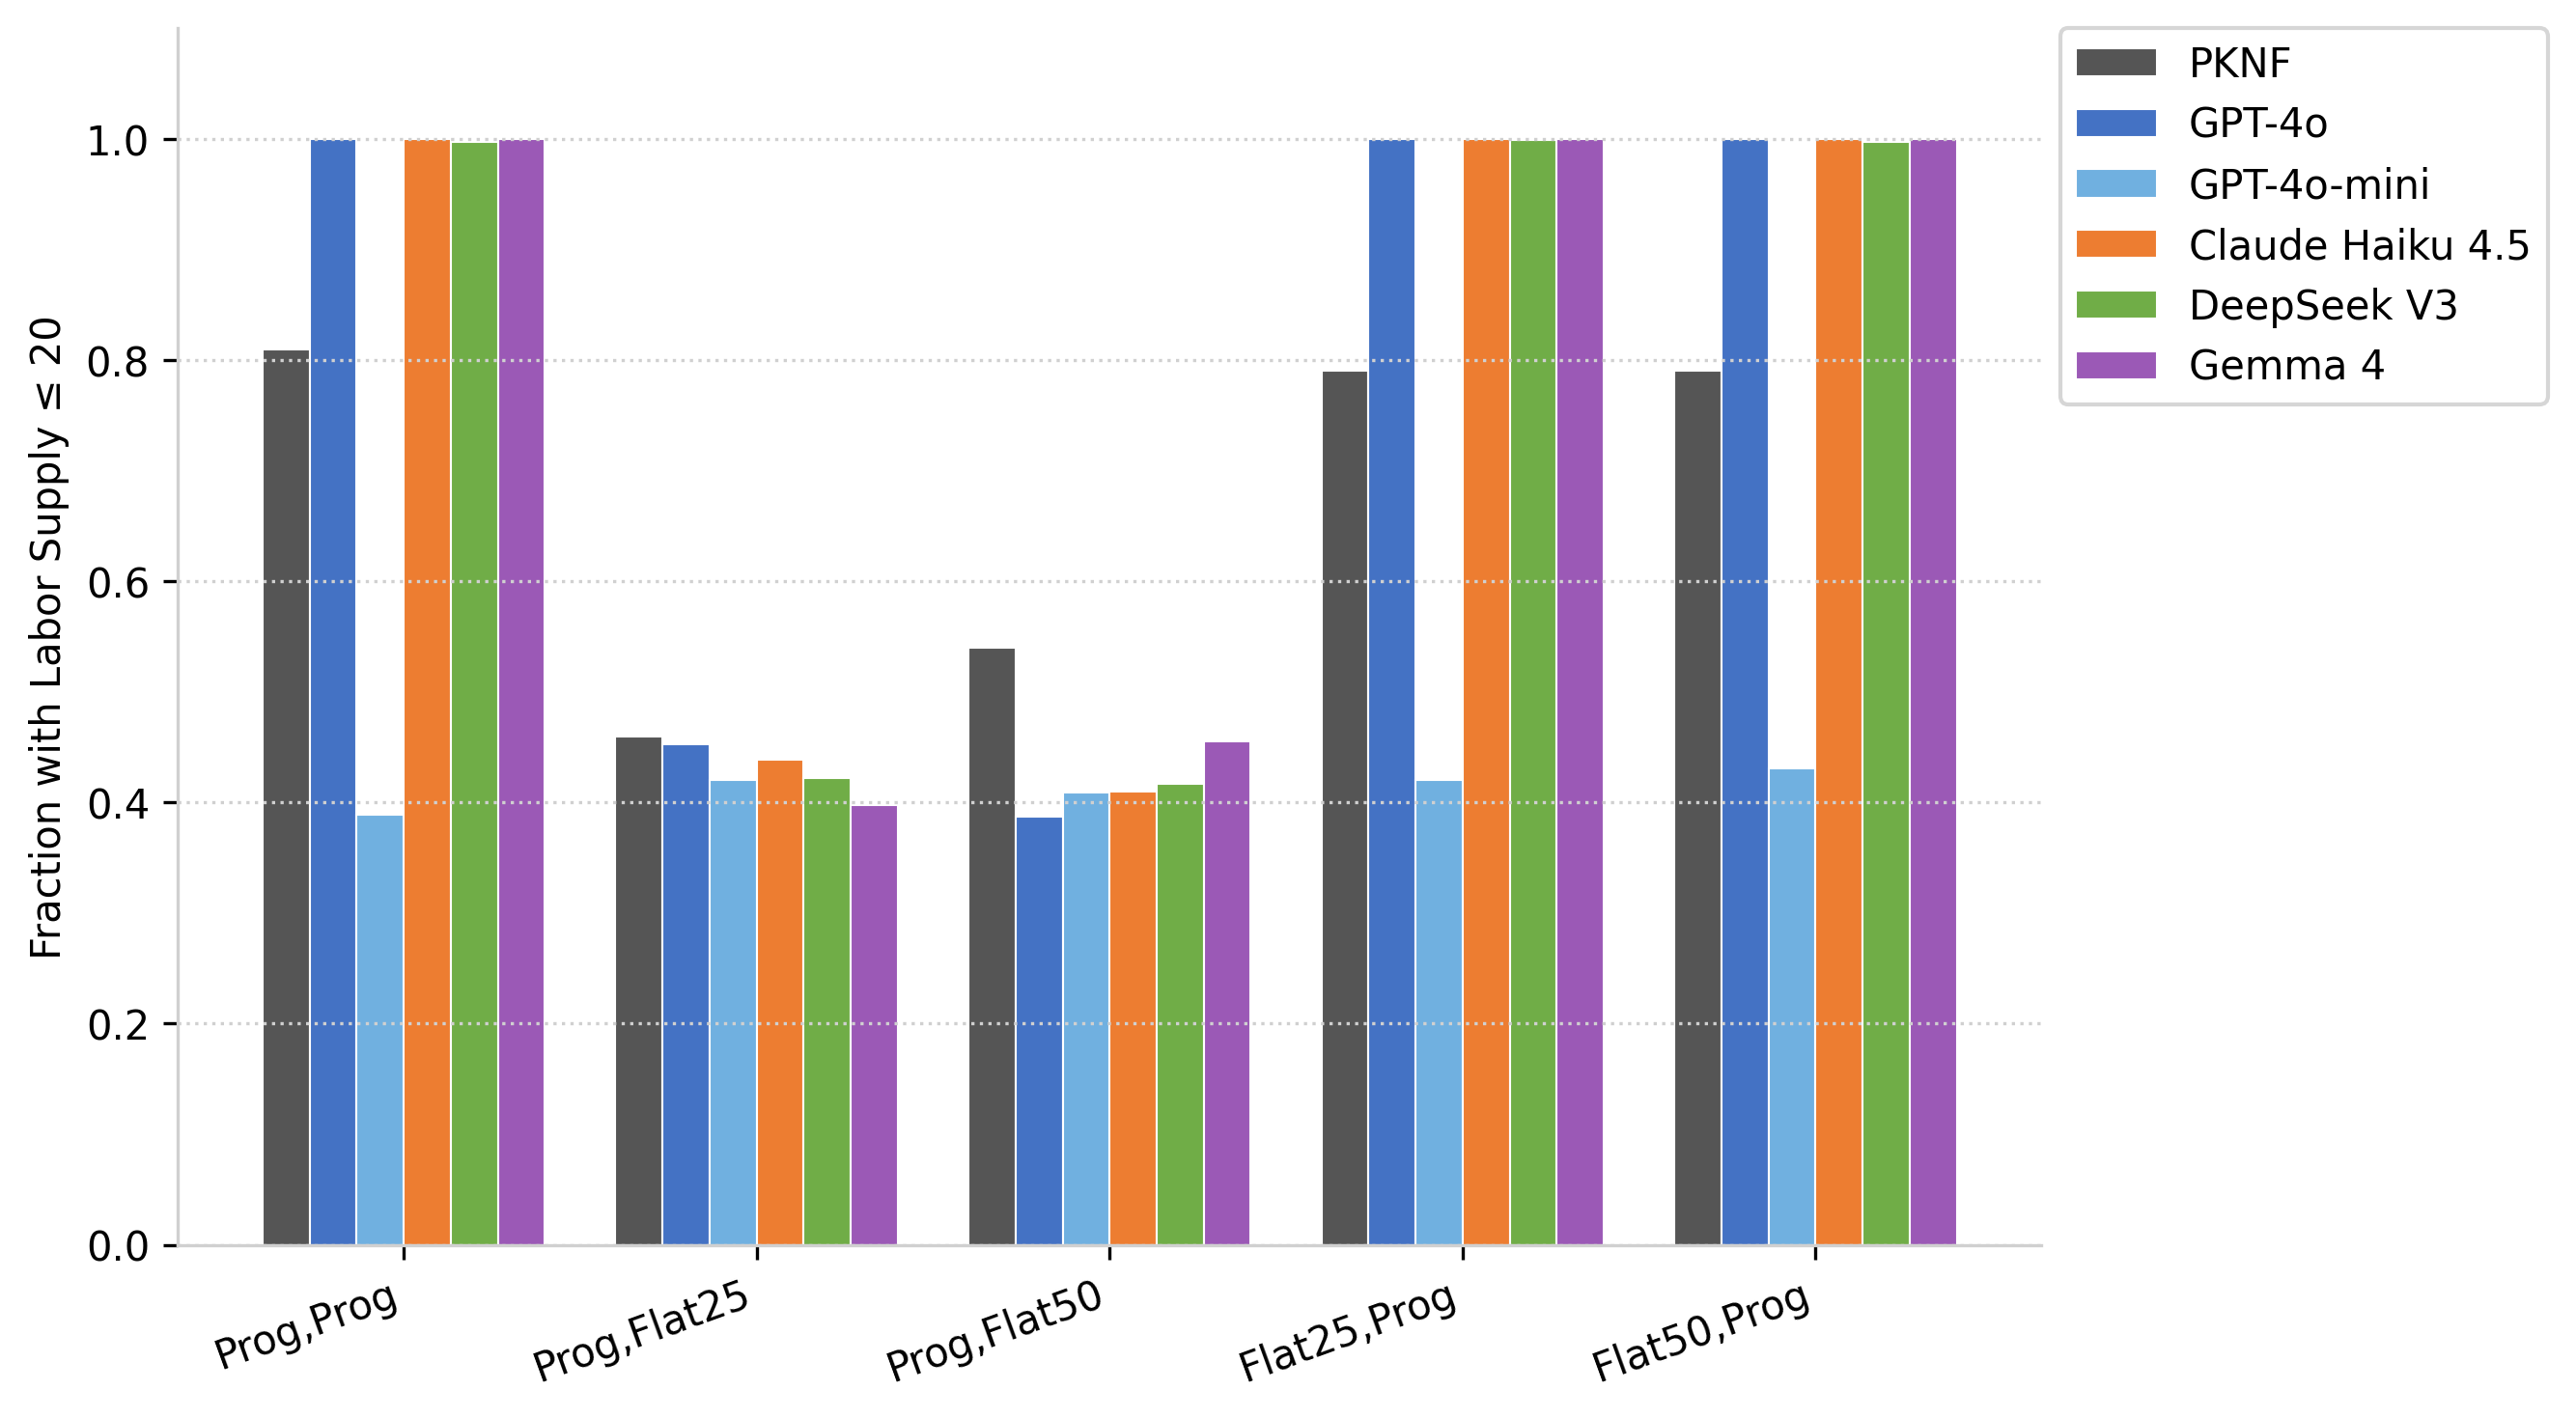
\includegraphics[width=0.55\textwidth]{images_tables//pknf_all_models_25pct_50pct_table5_bar_post.png}
    	}
        \caption{Fraction of subjects with labor supply $<$ 20:}
        \label{fig:LabSupply}
    \end{figure}


Since the notch binds at a labor supply above 20 units, it's useful to decompose the responses by the labor endowment of respondents. Those whose maximum endowment is less than 20 would not have any reason to change behavior in the presence of a notch. Figure \ref{fig:lab_supply_max} does just this, showing the mean labor supply under the 25\% to 50\% progressive tax schedule in gold and the flat tax of 25\% in blue, separating out respondents by their labor endowment (called ``maximum tasks'' in \cite{PKNF2024}).  In both cases, we see no differences in labor supply between the flat tax and progressive systems for those with labor endowment of 20 or less, but observe growing differences in labor supply across the two systems as the labor endowment grows from 20 to 30.

    \begin{figure}[h]
    \caption{Labor supply by ``Potential Income''}
    \label{fig:lab_supply_max}
     \subfigure[Pfeil et al. (2025)]{
     % \vspace{6mm} HAVING trouble getting these lined up.  Should we just recreate PKNF?
     \centering
   	 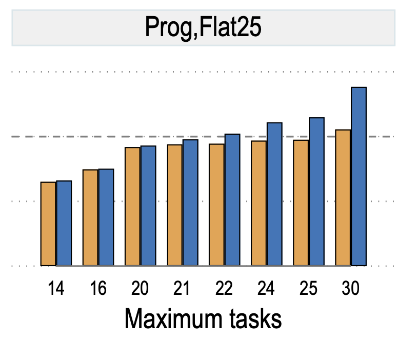
\includegraphics[width=0.47\textwidth]{images_tables/PKNF_Fig2b.png}
	}
    \subfigure[LLM: GPT-4o]{
    \centering
   	 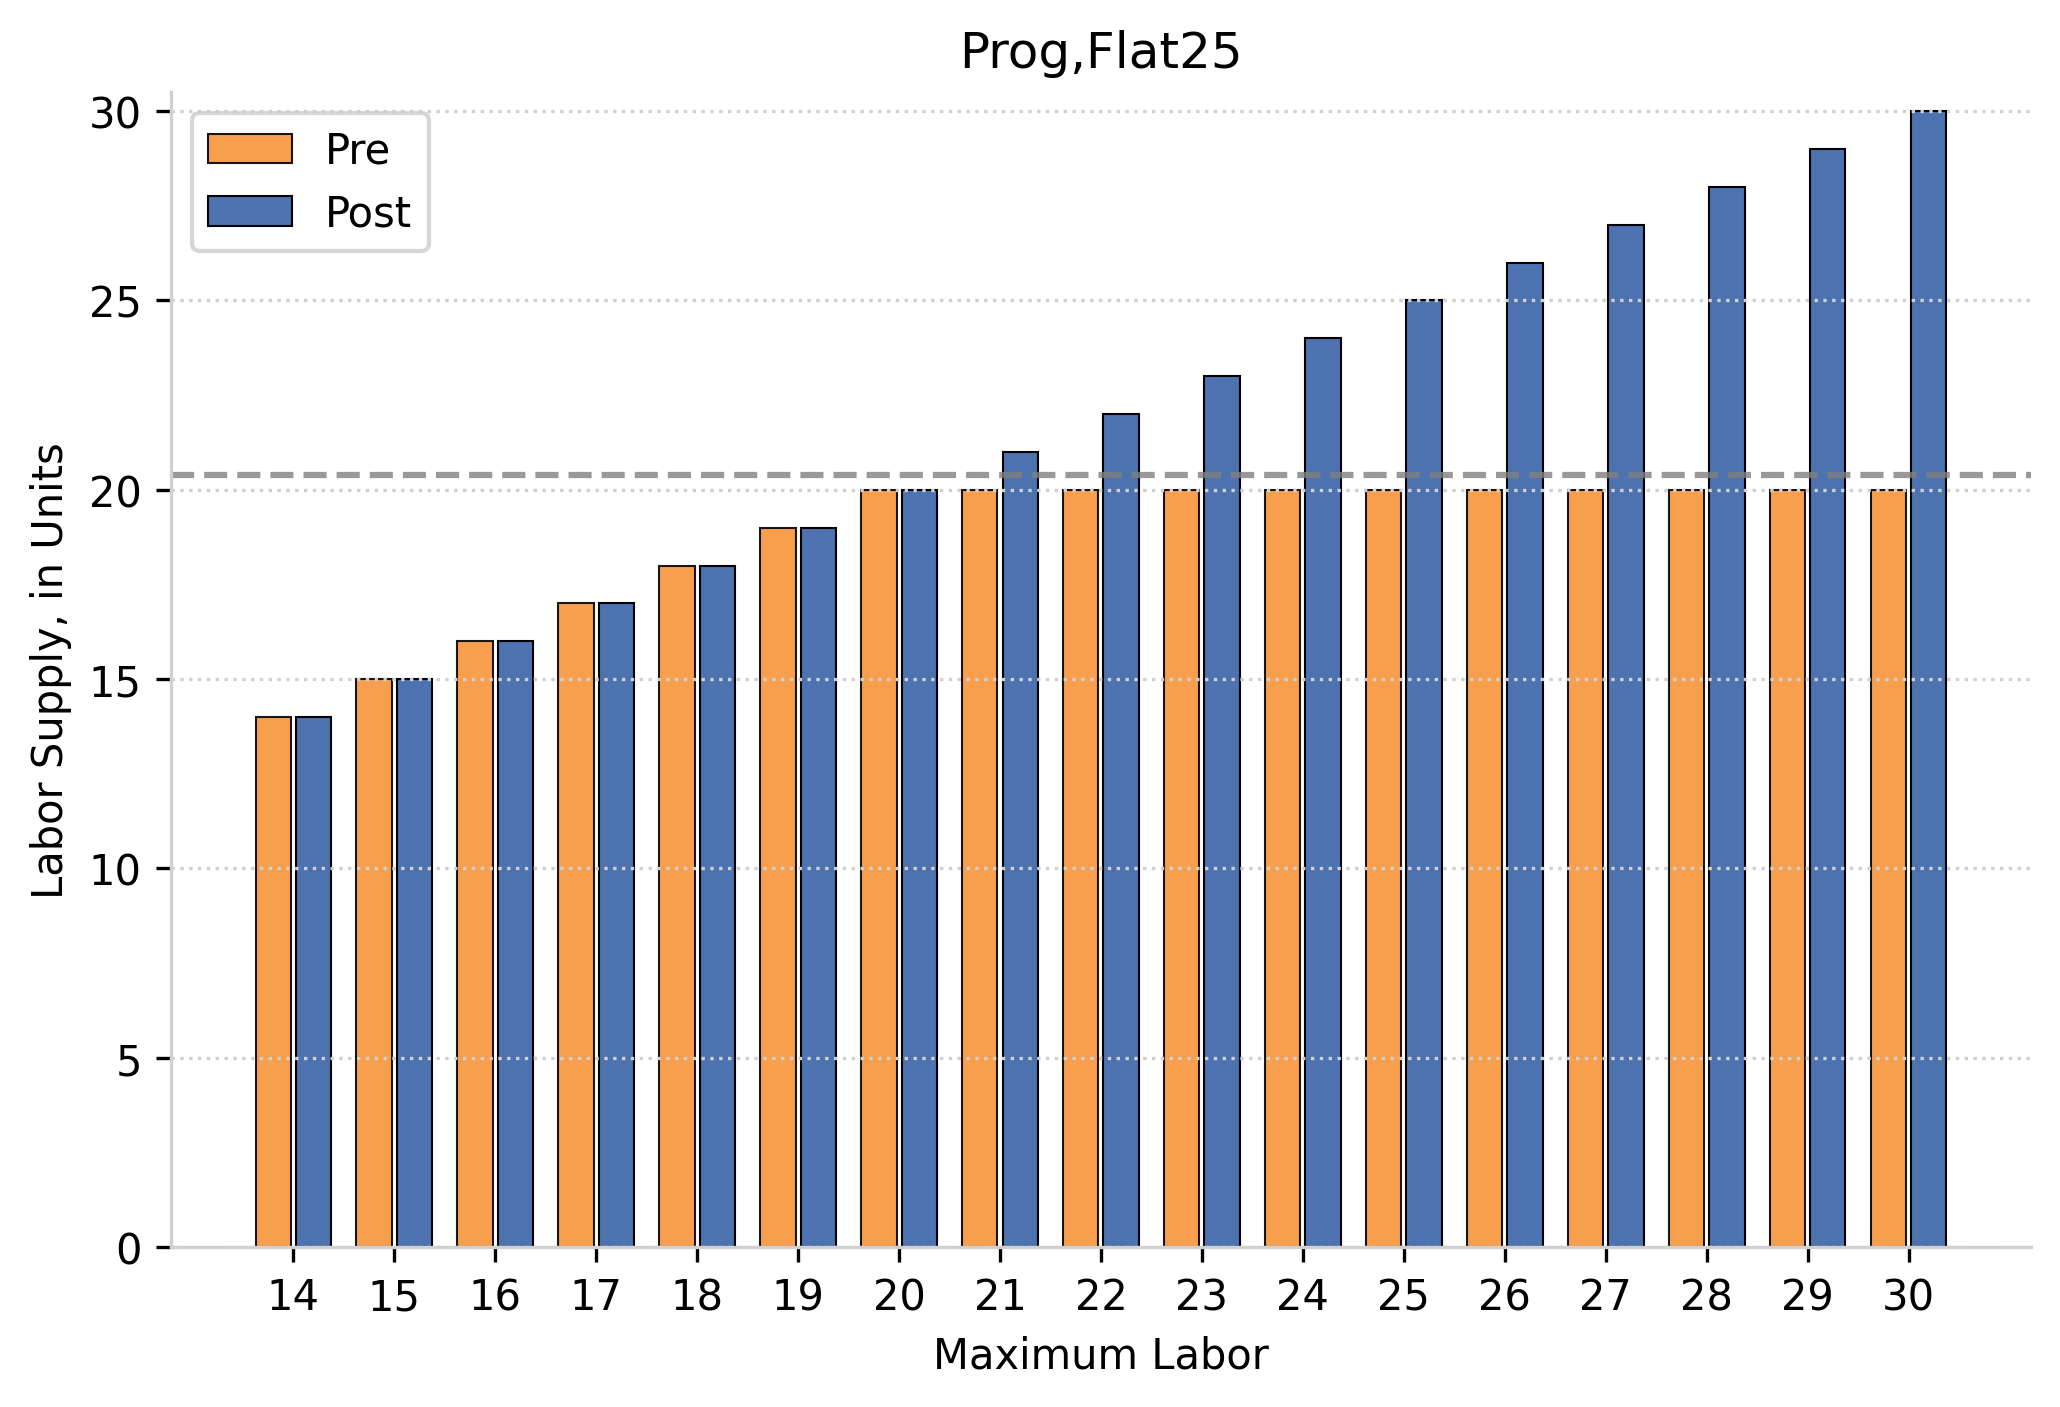
\includegraphics[width=0.47\textwidth]{images_tables/pknf_gpt-4o_25pct_50pct_fig2_3.png}
	}
    \small{Figure decomposes responses by the labor endowment of agents by showing the mean labor supply for the human study (left) and our replication using LLMs (right). Responses for the 25\% to 50\% progressive tax schedule are shown in gold and those for the flat tax of 25\% in blue. Respondents are separated out by their labor endowment in the post period.}
    \end{figure}
    

Next, we present the responses by treatment and round.  This illustrates if there is any learning over time as the game progresses and how respondents change when moving from a flat to progressive or progressive to flat, as well as from systems with higher or lower marginal tax rates. Figure \ref{fig:lab_supply_round} summarizes the results for \cite{PKNF2024} and for our replication using GPT-4o. The results for human subjects do not show clear patterns in behavior across rounds within treatment, but one can clearly see increases (decreases) in labor supply when moving away from (to) the progressive tax schedule.  In the right panel, we have the results from the LLM simulations.  These are much less noisy and clearly show no changes in behavior across rounds within a treatment.  The changes in labor supply when moving from (to) the progressive system are very sharp and in the same direction as human subjects.  It's notable that under the flat tax systems, labor supply from the LLMs is nearly 100\% of the players' labor endowment, while human subjects' labor supply under these systems is in the 85-93\% range.

    \begin{figure}[h]
    \centering
    \caption{Labor Supply Responses by Treatment} 
    \label{fig:lab_supply_round}
     \subfigure[Pfeil et al. (2025)]{
   	 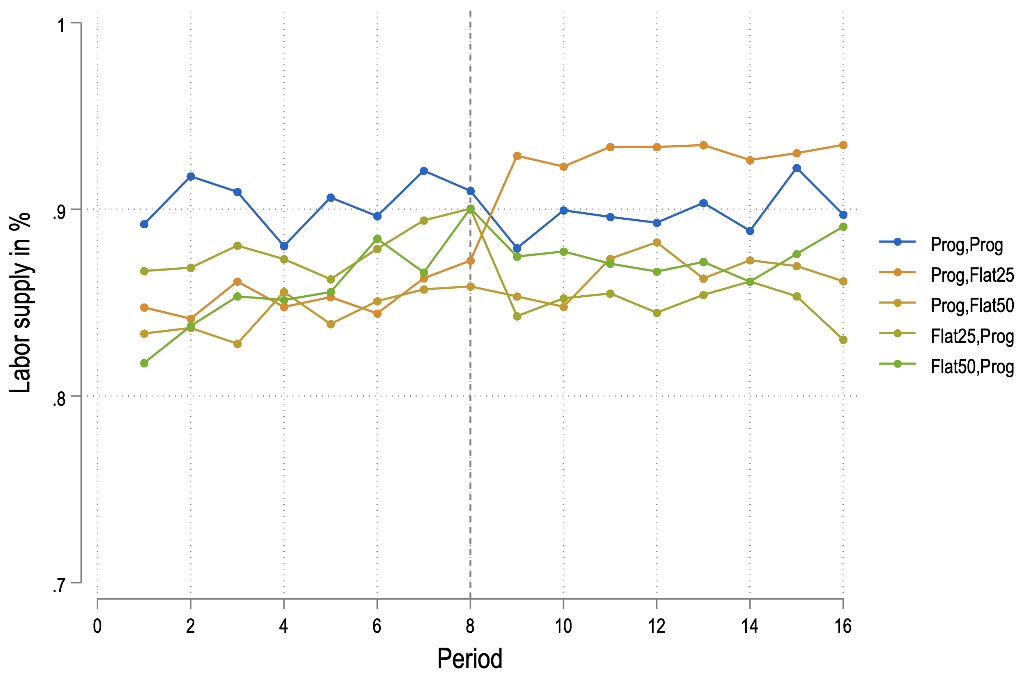
\includegraphics[width=0.47\textwidth]{images_tables/PKNF_Fig4.png}
	}
    \subfigure[LLM]{
   	 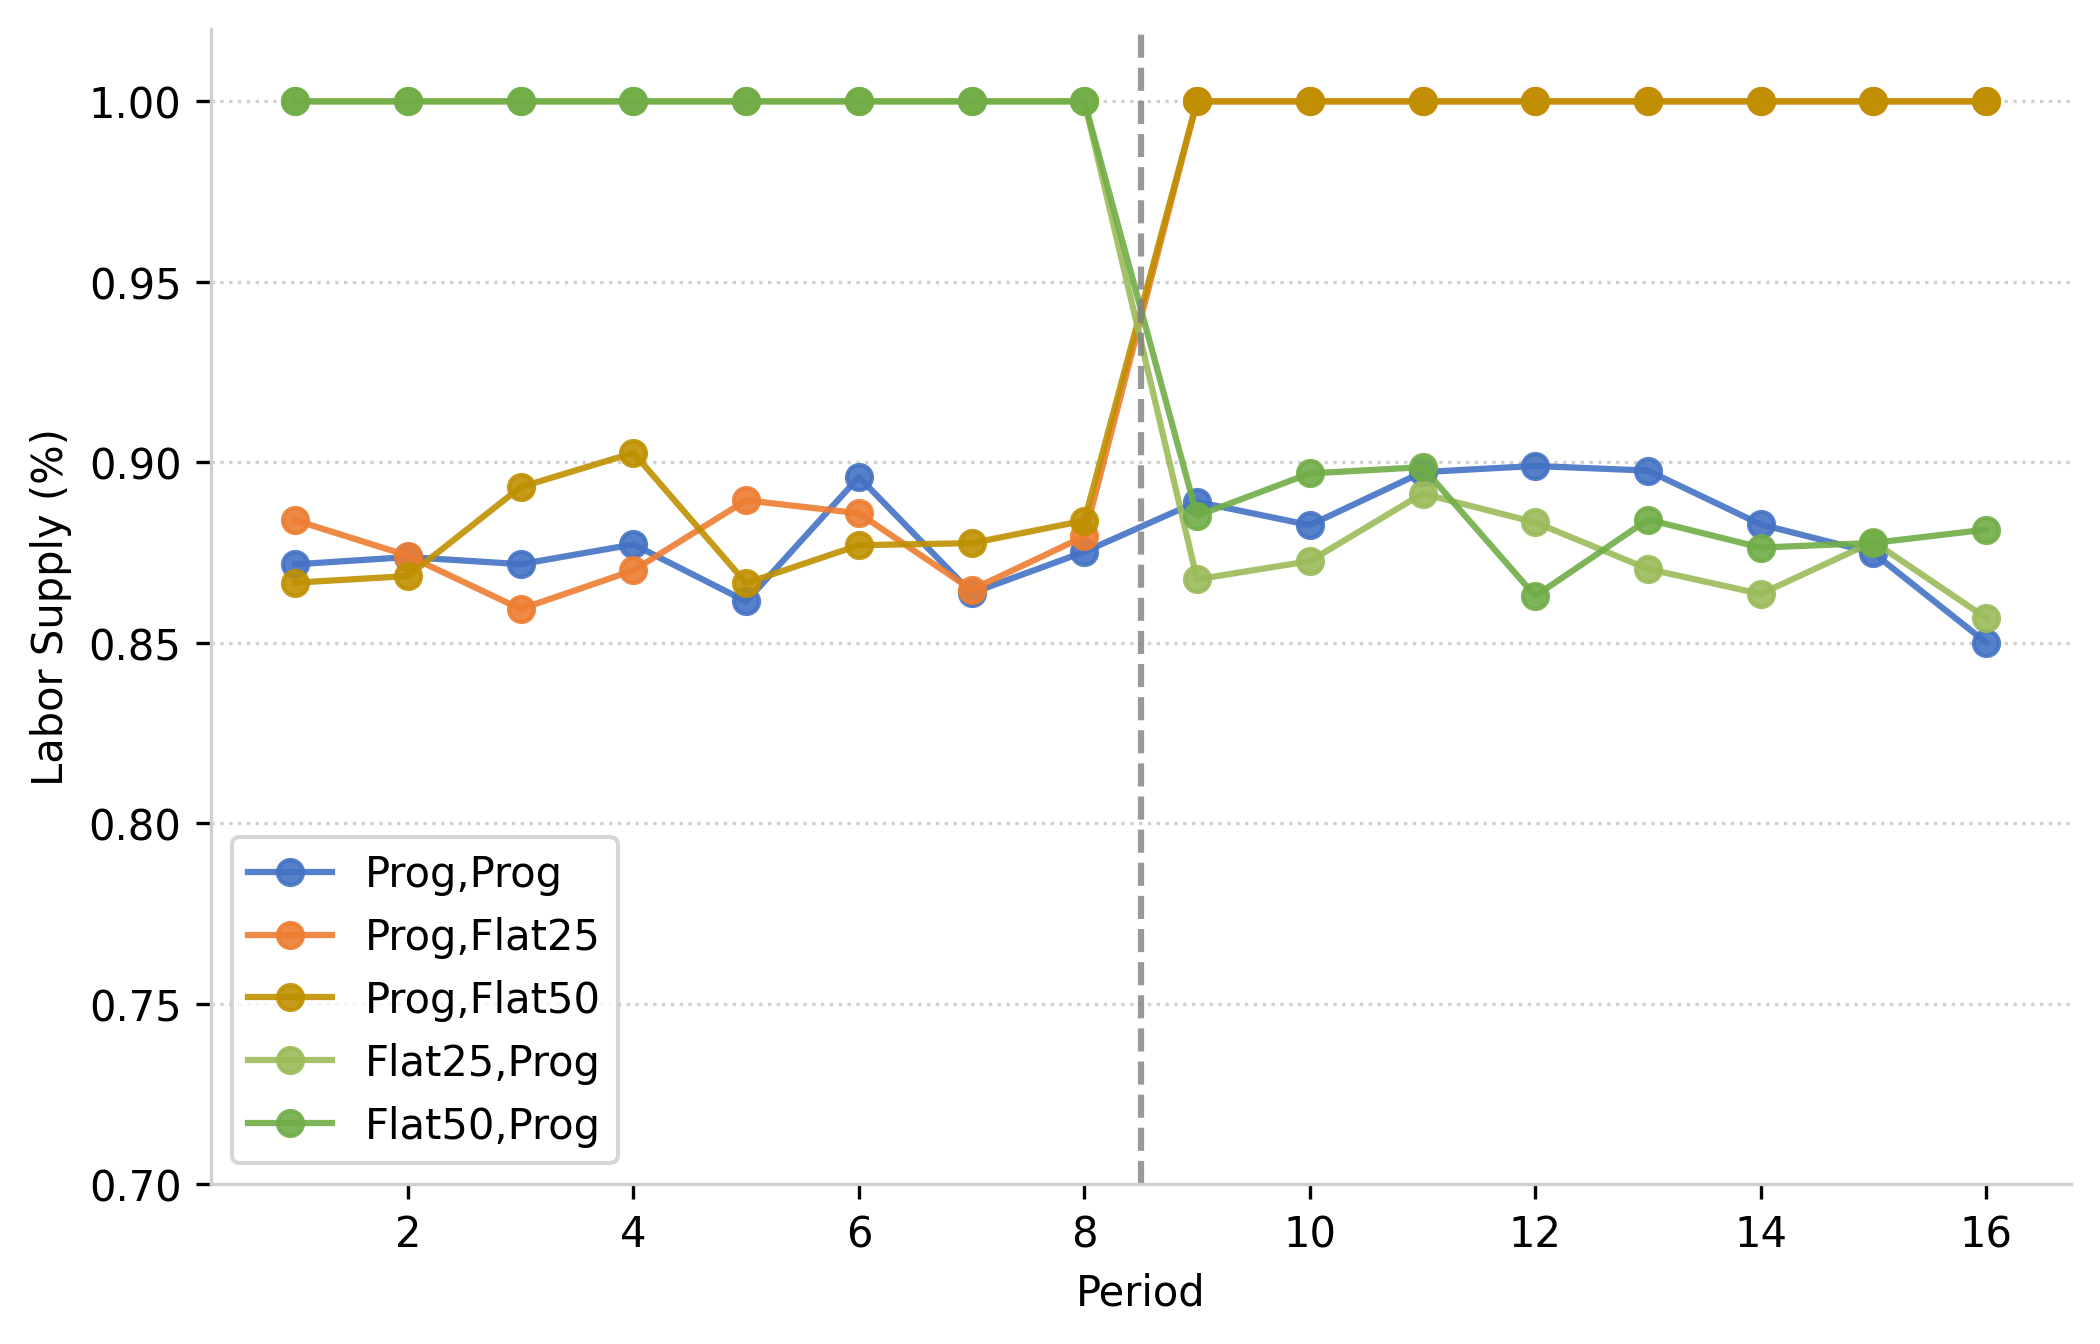
\includegraphics[width=0.47\textwidth]{images_tables/pknf_gpt-4o_25pct_50pct_fig4.png}
	}
    \small{Figure displays responses by treatment and round for \cite{PKNF2024} (left) and for our replication using GPT-4o (right). Additional results can be found in Appendix \ref{sec:AppendixA}.}
    \end{figure}

Finally, we present differences-in-differences estimates of the labor supply responses from the LLM. In this model, we regress labor-supply units on indicators for the last 8 rounds (post), treatment (which is the change from a progressive tax to a flat tax), and the interaction of the post rounds with treatment.  The sample includes observations from a control group where all 16 rounds were played under the progressive tax system and a treated group where the first eight rounds were played under a progressive tax system and the last eight under a flat tax of 25\%.  Differences-in-differences estimates from PKNF and from our LLM simulations are shown in Table \ref{tab:DD_estimates}.  The insignificant post indicator suggests that neither humans nor the LLMs are changing behavior in later rounds as a result of learning.  The exception to this is the GPT-4o model which has a significant ``post'' coefficient.  The treated indicator (``Prog,Flat25'') is significant in column 1, suggesting slightly lower labor supply across all rounds from human participants in the treated group. For the AI simulations, this coefficient is statistically indistinguishable from zero.  The coefficient of interest is the interaction of the post and treatment indicators and it's positive and significant in both the \cite{PKNF2024} study and the LLM replications of that study, with the exception of the GPT-4o-mini results where there is so little variation across simulations that the constant absorbs almost all the variation.  The coefficients suggest that labor supply increases by 8.3\% among the human participants and 11.4 to 12.4\% in the LLMs after moving from the progressive tax schedule to a 25\% flat tax, with the average effect when pooling all LLM simulations (including GPT-4o-mini) being an effect of 9.8\%.  We cannot reject the hypothesis that humans and LLMs are responding to the same degree to the change in the tax schedule at the 5\% level.

    \begin{table}
    \centering
    \caption{Differences-in-Differences Estimates}
    \label{tab:DD_estimates}
    \begin{tabular}{llllllll}
\toprule
 & PKNF & GPT-4o & GPT-4o-mini & Claude Haiku 4.5 & DeepSeek V3 & Gemma 4 & Pooled LLMs \\
\midrule
Post & -0.007 & 0.010 & 0.001 & -0.006 & 0.002 & 0.009 & -0.004 \\
 & (0.006) & (0.005) & (0.000) & (0.005) & (0.005) & (0.005) & (0.002) \\
Treated & -0.052 & 0.002 & 0.000 & 0.002 & 0.002 & -0.004 & 0.002 \\
 & (0.022) & (0.005) & (0.000) & (0.006) & (0.006) & (0.006) & (0.002) \\
Post*Treated & 0.083 & 0.114 & -0.000 & 0.124 & 0.120 & 0.118 & 0.098 \\
 & (0.009) & (0.008) & (0.001) & (0.007) & (0.008) & (0.007) & (0.003) \\
Constant & 0.947 & 0.874 & 0.999 & 0.881 & 0.876 & 0.877 & 0.905 \\
 & (0.055) & (0.004) & (0.000) & (0.004) & (0.004) & (0.004) & (0.002) \\
N & 3344 & 3200 & 3121 & 3200 & 3187 & 3190 & 15898 \\
R-squared & 0.035 & 0.200 & 0.001 & 0.232 & 0.231 & 0.235 & 0.157 \\
\bottomrule
\end{tabular}

    \end{table}

\subsection{The Elasticity of Taxable Income}
The above results show that the labor supply responses measured in the \cite{PKNF2024} study are qualitatively reproduced in the AI simulations, but that the quantitative estimates generally show larger labor supply responses to changes in taxes than what were measured in the laboratory.  However, \cite{PKNF2024} don't provide estimates of the elasticity of taxable income in their study.  We extend their work and estimate ETIs from the LLM responses using a bunching estimator.

    \begin{figure}
    \centering
    \caption{Distribution of Pre-Tax Income: GPT-4o}
    \label{fig:Income_density}
    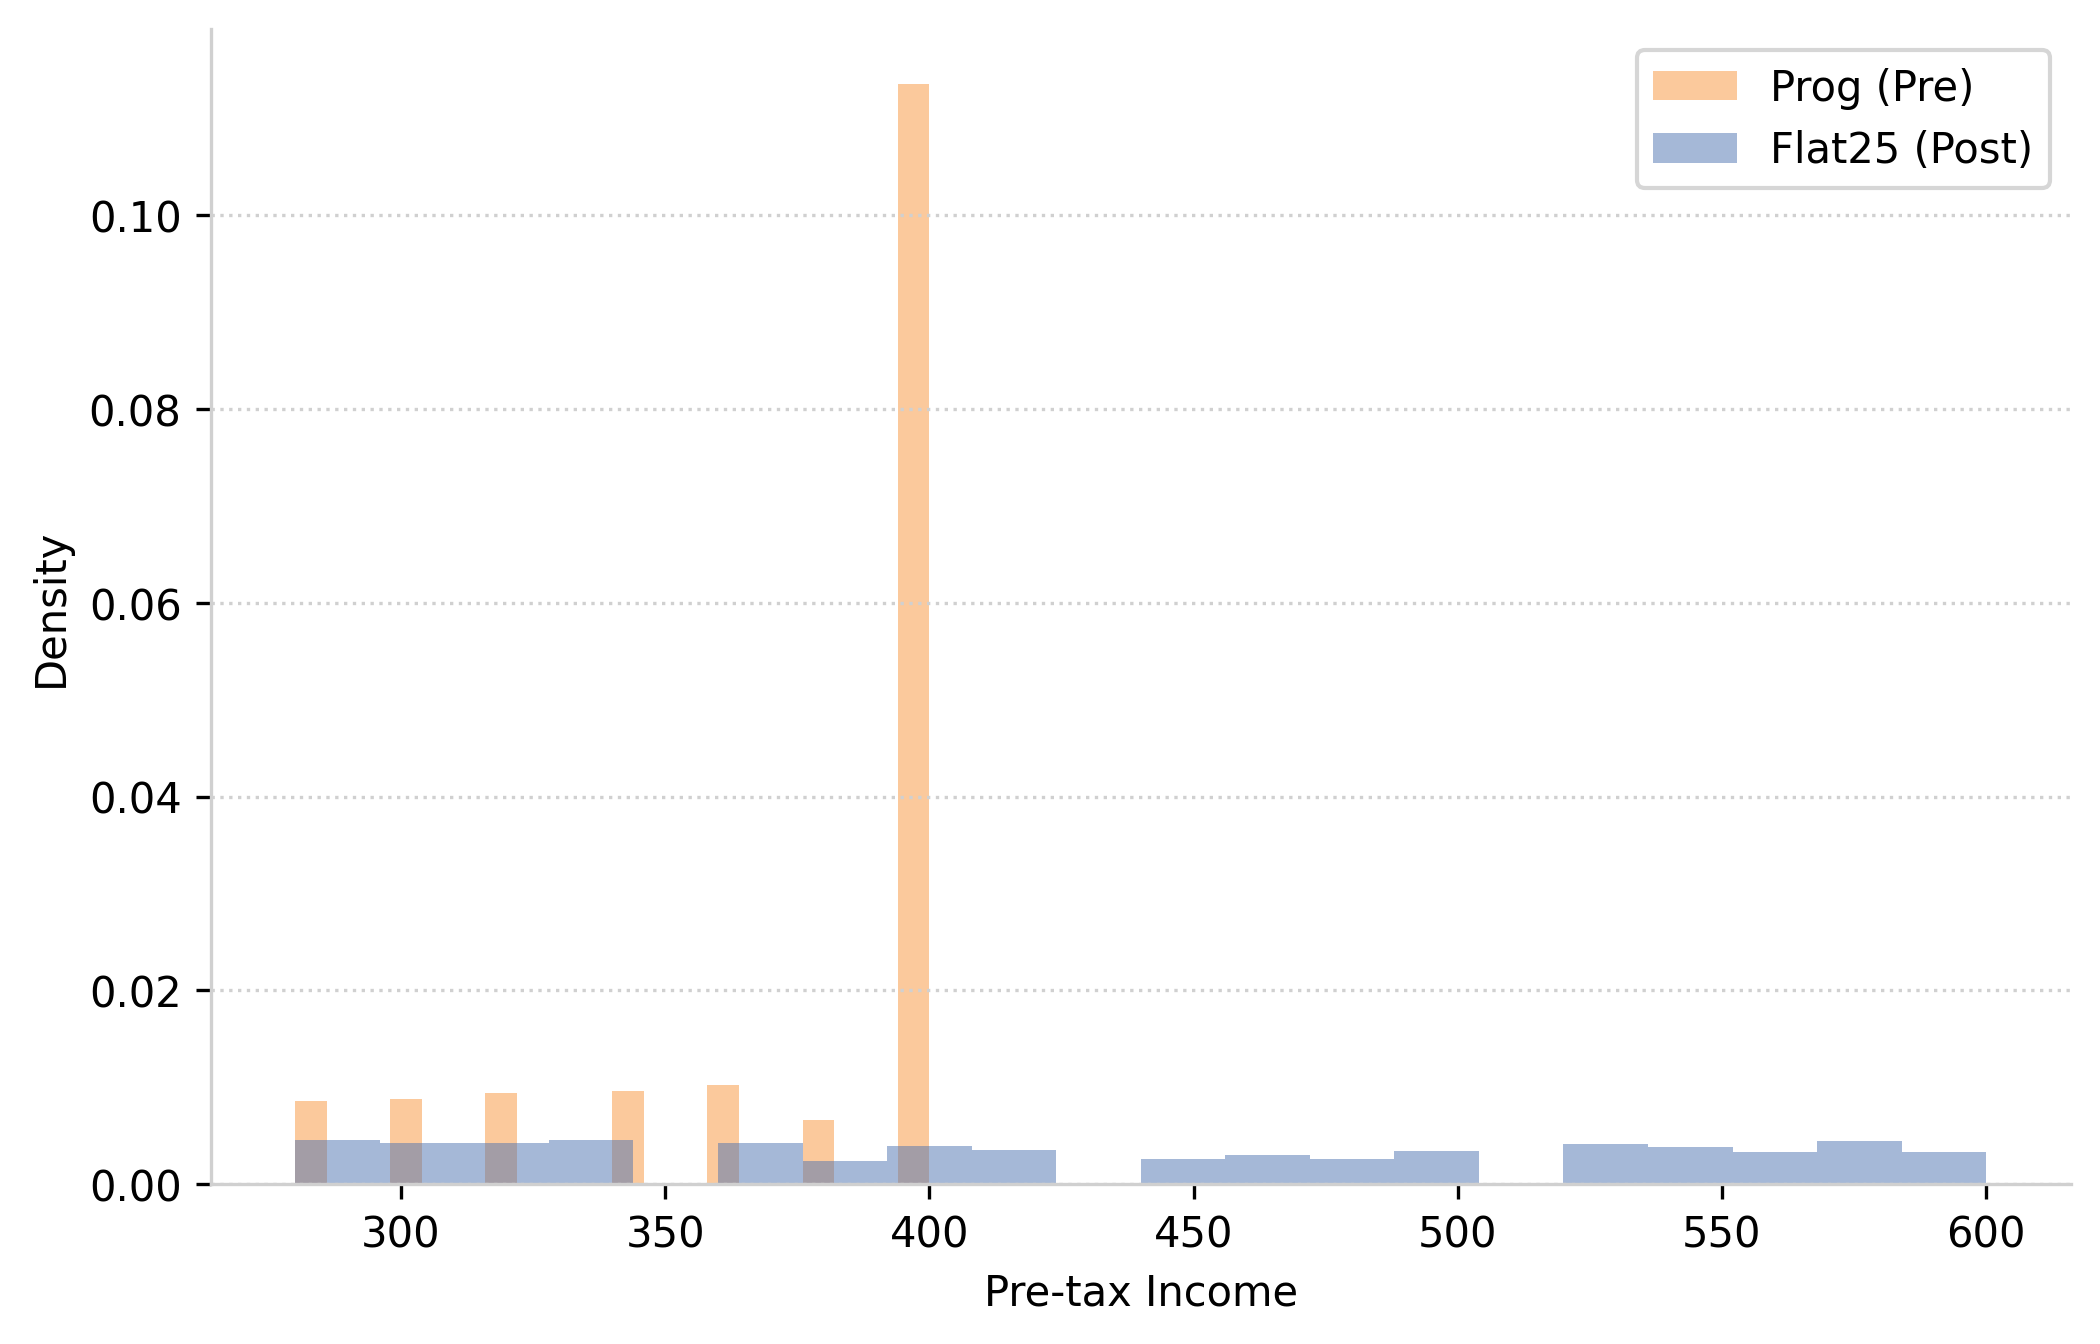
\includegraphics[width=0.8\textwidth]{images_tables/pknf_gpt-4o_25pct_50pct_bunching.png}
    \end{figure}

 
Figure \ref{fig:Income_density} shows the density of pre-tax income under a flat 25\% tax and the progressive tax system.  The distribution under the flat tax is relatively uniform, mirroring the draws of labor endowments. On the other hand, the distribution of pre-tax income under the progressive tax schedule displays a large mass at 400, which is the threshold above which the higher tax rate is applied. There are no LLM simulations with pre-tax income above this level, representing an area with a missing mass.  Ideally, we'd estimate that range of pre-tax income over which the missing mass exists.  But in the setup of \cite{PKNF2024} the dominated region (which is a subset of the area where theory predicts a missing mass) extends up to 600, which is the maximum earnings any player can have. 

With this issue in mind, we report two ETI estimates. The first is a \textit{structural lower bound} following \citet{KlevenWaseem2013}: because no rational agent should locate in the dominated region, all agents whose counterfactual income lies within $\Delta z^*$ of $z^*$ will bunch at $z^*$. The implied lower bound is
  \begin{equation}
      e_{\min} = \frac{\Delta z^*/z^*}{\left[(\tau_2-\tau_1)/(1-\tau_2)\right]},
      \label{eq:eti_lb}
  \end{equation}
  which equals 0.5 under the 50\% top rate. This bound is a fixed function of the tax schedule parameters and carries no sampling uncertainty. The second estimate is \textit{data-driven}: we measure excess bunching at $z^*$ as the difference between the fraction of eligible observations at exactly $z^*$ under the progressive schedule and the counterfactual density estimated from flat-schedule observations in a symmetric window of $\pm 40$ ECU around $z^*$.\footnote{We restrict to rounds in which the agent's labor endowment strictly exceeds $z^*/w = 20$ units, so that bunching at $z^*$ represents a genuine behavioral choice rather than a ceiling effect.}
  
  The implied average income adjustment $\widetilde{\Delta z}$ is then capped at $\Delta z^*$ and converted to an ETI via equation~\eqref{eq:eti_lb}. Standard errors and 95\% confidence intervals for the data-driven estimate are obtained by bootstrap (1{,}000 draws), resampling progressive and flat eligible observations independently with replacement. Table \ref{tab:ETI_estimates50} reports ETI estimates from both methods and for each model under the simulations with a top marginal tax rate of 50\%.  Given that all models except for GPT-4o-mini show perfect bunching, the elasticity estimates from the data-driven approach are identical to the structural lower bound.

  \begin{table}
    \centering
    \caption{Elasticity of Taxable Income Estimates: 50\% top rate}
    \label{tab:ETI_estimates50}
    \begin{tabular}{lll}
\toprule
 & Structural LB & Data-Driven ETI \\
Model &  &  \\
\midrule
GPT-4o & 0.500 & 0.500 \\
 &  & [0.500, 0.500] \\
GPT-4o-mini & 0.500 & 0.000 \\
 &  & [0.000, 0.000] \\
Claude Haiku 4.5 & 0.500 & 0.500 \\
 &  & [0.500, 0.500] \\
DeepSeek V3 & 0.500 & 0.500 \\
 &  & [0.500, 0.500] \\
Gemma 4 & 0.500 & 0.500 \\
 &  & [0.500, 0.500] \\
\bottomrule
\end{tabular}

    \end{table}

To address the challenge of identifying the ETI from the \citet{PKNF2024} setup, we consider an alternative design in which the top marginal tax rate is set to 40\% rather than 50\%. Under this alternative parameterization, the dominated region no longer extends to the maximum labor endowment of 30 (which has earnings of 600), allowing for observed labor supply responses beyond the dominated region to the right of the notch threshold. Figure~\ref{fig:Income_density_alt} shows the resulting income distribution. Even with the 40\% top rate, we still find no simulations where pre-tax labor income is above the notch. Under this parameterization, the lower bound elasticity is 0.25.  Table \ref{tab:ETI_estimates40} presents the ETI estimates from both the lower bound method and the empirically driven method for simulations with a top marginal tax rate of 40\%.  Given that all models except for GPT-4o-mini show perfect bunching, the elasticity estimates from the data-driven approach are identical to the structural lower bound.  However, since the dominated region is smaller in this case, the lower bound elasticity is lower.

    \begin{figure}
    \centering
    \caption{Distribution of Pre-Tax Income: Alternative Parameterization (40\% Top Rate): GPT-4o}
    \label{fig:Income_density_alt}
    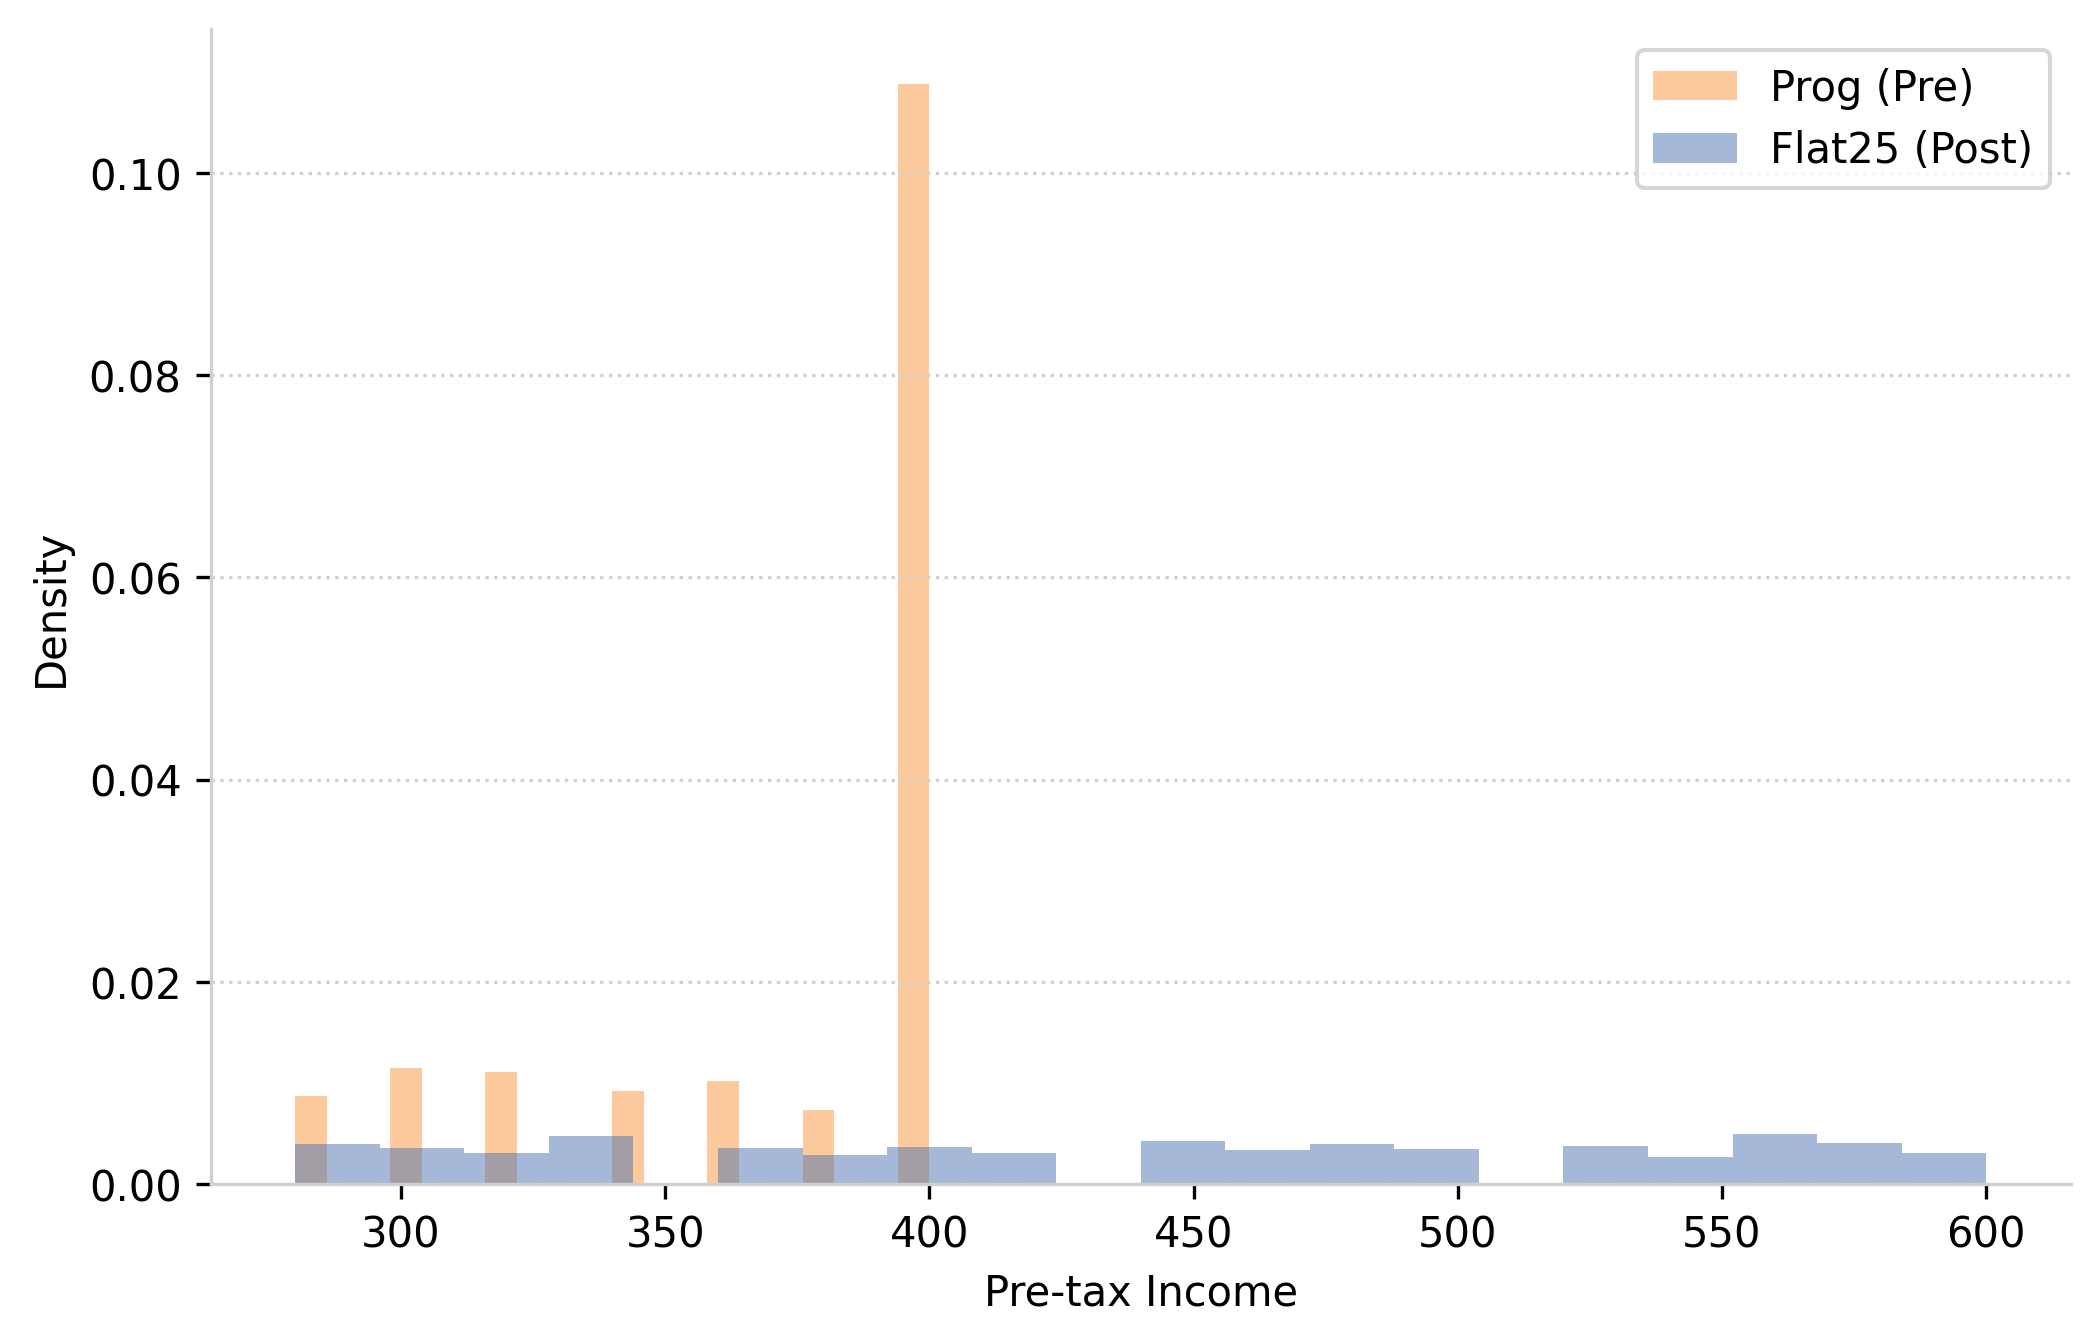
\includegraphics[width=0.8\textwidth]{images_tables/pknf_gpt-4o_25pct_40pct_bunching.png}
    \small{\\ Figure notes: Income distribution under the progressive tax schedule with a 40\% top rate (orange) and a flat 25\% tax (blue).}
    \end{figure}



    \begin{table}
    \centering
    \caption{Elasticity of Taxable Income Estimates: 40\% top rate}
    \label{tab:ETI_estimates40}
    \begin{tabular}{lll}
\toprule
 & Structural LB & Data-Driven ETI \\
Model &  &  \\
\midrule
GPT-4o & 0.250 & 0.250 \\
 &  & [0.250, 0.250] \\
GPT-4o-mini & 0.250 & — \\
 &  &  \\
Claude Haiku 4.5 & 0.250 & 0.250 \\
 &  & [0.250, 0.250] \\
DeepSeek V3 & 0.250 & 0.250 \\
 &  & [0.250, 0.250] \\
Gemma 4 & 0.250 & 0.250 \\
 &  & [0.250, 0.250] \\
\bottomrule
\end{tabular}

    \end{table}

\section{Conclusion}
\label{sec:Conclude}

This paper adds to a growing body of evidence that LLMs reproduce human behavior in economic contexts, extending that literature to a central parameter in public finance: the elasticity of taxable income. Across two distinct empirical settings, a seminal observational study and a controlled laboratory experiment, LLMs produce behavioral responses that are qualitatively, and often quantitatively, consistent with those of real taxpayers. However, LLMs are generally more responsive to marginal tax rate changes, suggesting LLMs do not fully internalize the frictions real taxpayers face.

The LLMs broadly reproduce the observational elasticity estimates of \cite{GruberSaez2002}, with an overall taxable income elasticity of 0.378 that closely matches their headline estimate of 0.400. However, results vary substantially across models:  ETIs range from 0.031 (GPT-4o) to 0.792 (Claude Haiku 4.5). Mean values also mask considerable heterogeneity within models. In terms of replicating variation in the ETI across income, the LLMs fall short: they show no change in ETI as taxpayer income changes.

In the replication of the \cite{PKNF2024} experimental study, the LLMs qualitatively reproduce human subjects' labor supply responses, including bunching below the notch, sharp reactions to the reform, and a statistically indistinguishable difference-in-differences estimate of the effects of tax reforms on labor supply. However, the LLMs respond more strongly and with far less noise, consistent with them perceiving the tax incentives with less friction than real participants do.

LLMs are low-cost and flexible. Simulations with LLMs may complement experimental and observational methods as they are capable not only of replicating existing findings but of extending them. For example, we were able to recover ETI estimates from an experimental design that did not originally report them and probe alternative parameterizations to those tested with human subjects. At the same time, the substantial heterogeneity across models and the sensitivity of identification to experimental design counsel caution: validation across multiple LLMs, and an understanding of sensitivity to prompt engineering, remain prerequisites before LLM-simulated behavior can credibly inform tax policy analysis. Our results also point to strong tendencies for LLM responses to be more strongly-optimizing than human responses to a changing tax system.

Several important questions remain, such as understanding the sensitivity of our results to prompt engineering and understanding how these models change over time.  For example, previous work with earlier versions of the GPT and Claude models showed a smaller degree of optimizing behavior, more similar to humans.  Others, such as \cite{NBERw34745}, have documented similar increases in rational, strategic responses in later generation LLMs. Our next steps are to further explore prompting LLMs in this context to more accurately replicate human behavior from LLMs. We then hope to further explore heterogeneity (e.g., by income, sex, and itemization status) and the nature of the responses to marginal tax rates (e.g., capital gains realizations) as ways to further research on taxation using LLMs.

\newpage
\bibliography{references.bib}

\newpage
\appendix

% For Figures
\setcounter{figure}{0}
\renewcommand{\thefigure}{A.\arabic{figure}}

% For Tables
\setcounter{table}{0}
\renewcommand{\thetable}{A.\arabic{table}}

% For Equations
\setcounter{equation}{0}
\renewcommand{\theequation}{A.\arabic{equation}}

\section{Results for other LLMs not reported in main text}
\label{sec:AppendixA}

\subsection{Labor Supply Responses by Treatment: All Models}
    \begin{figure}[h]
    \centering
    \caption{Labor Supply Responses by Treatment} 
    \label{fig:lab_supply_round_all_models}
     \subfigure[GPT-4o-mini]{
   	 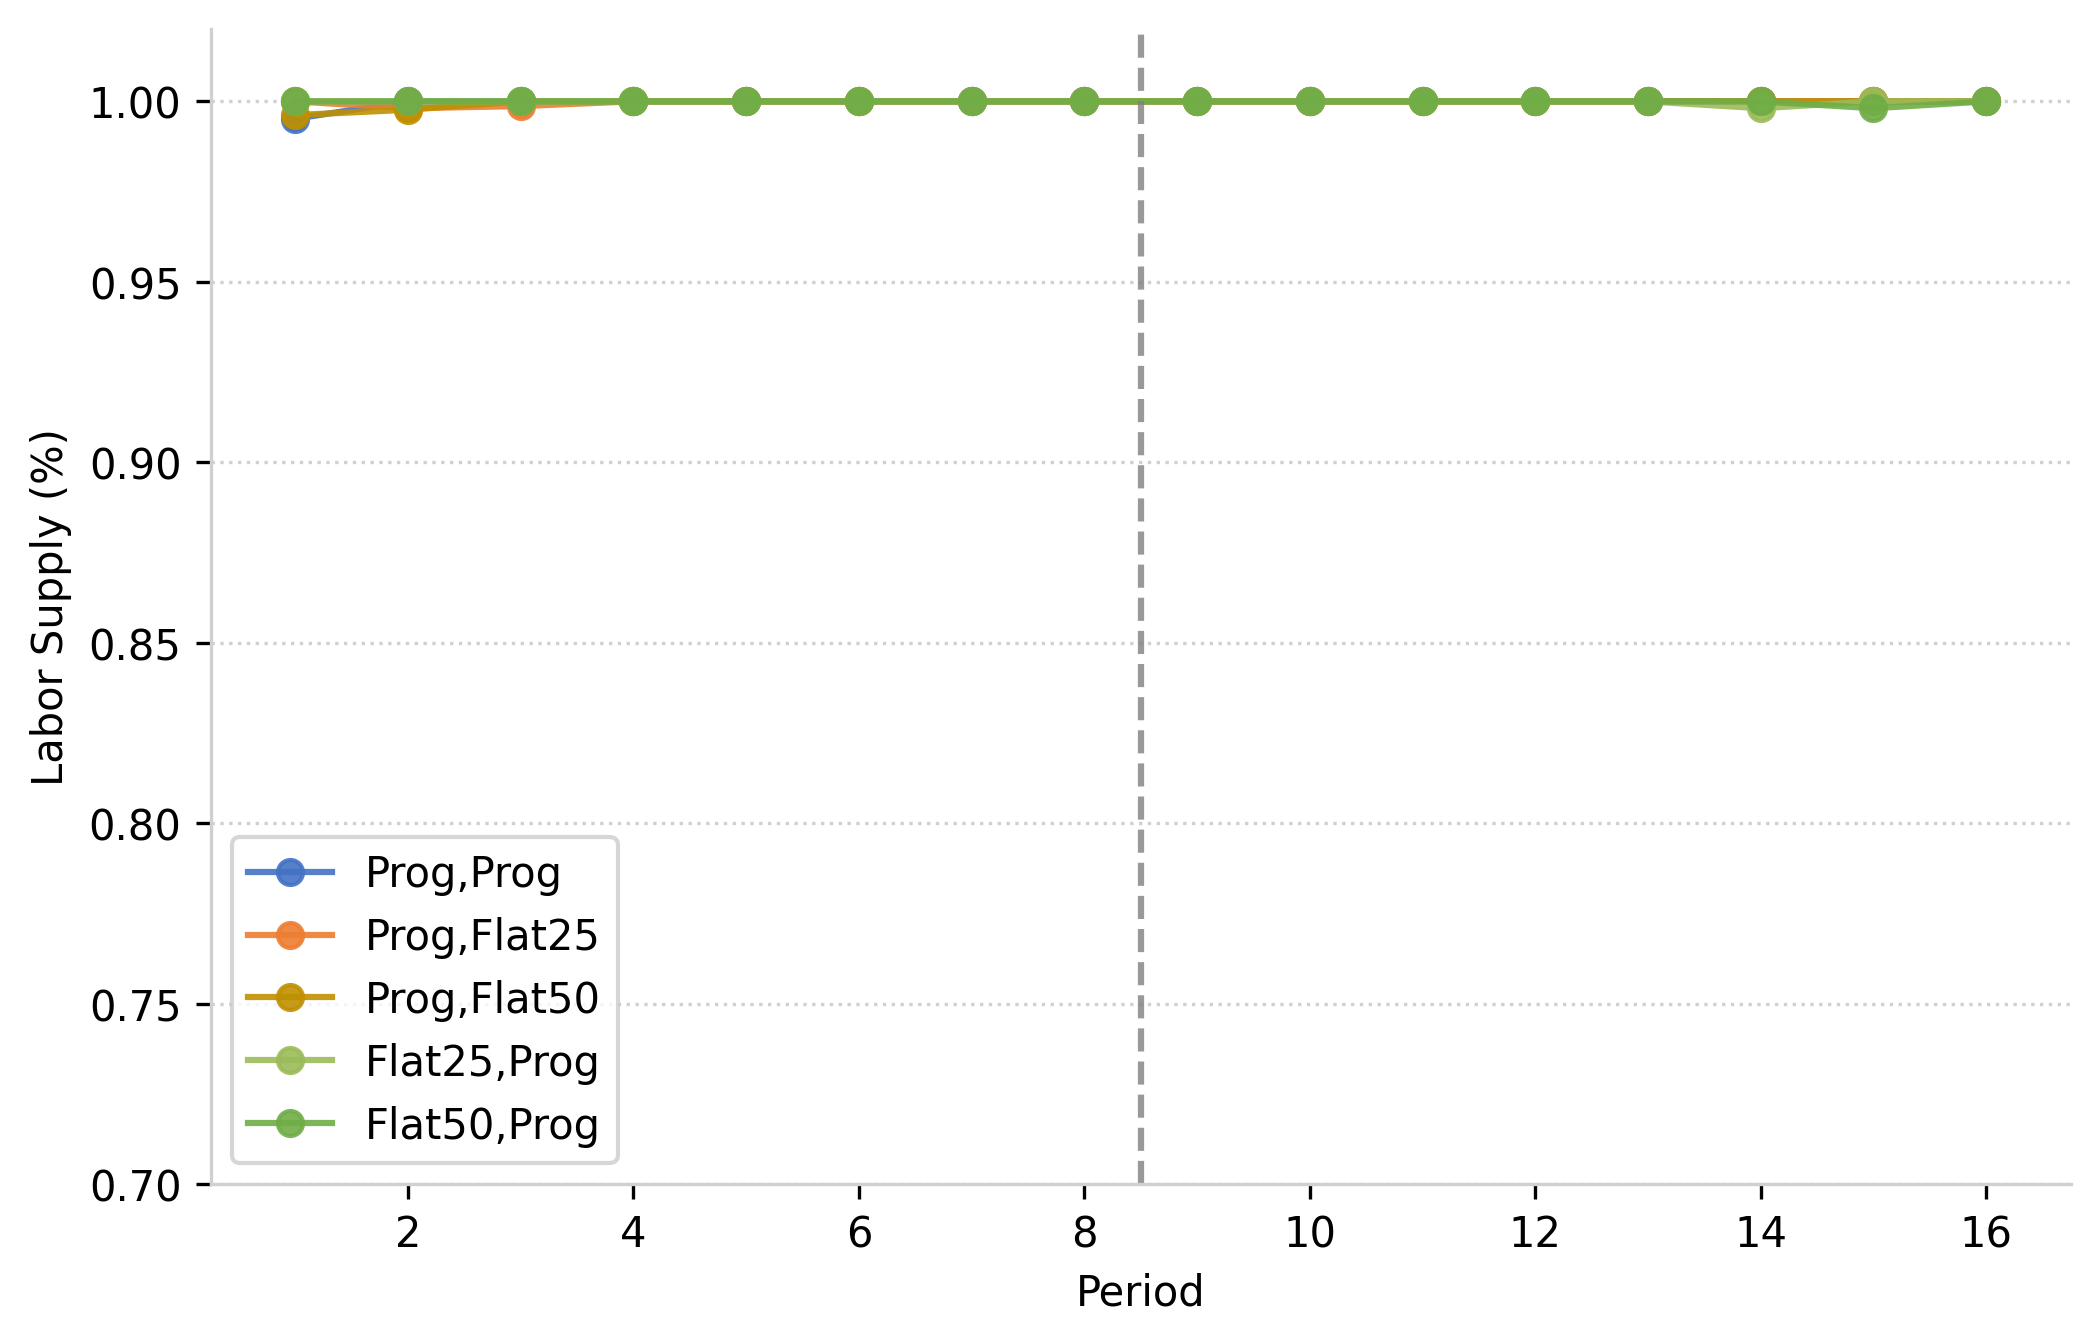
\includegraphics[width=0.47\textwidth]{images_tables/pknf_gpt-4o-mini_25pct_50pct_fig4.png}
	}
    \subfigure[Claude Haiku 4.5]{
   	 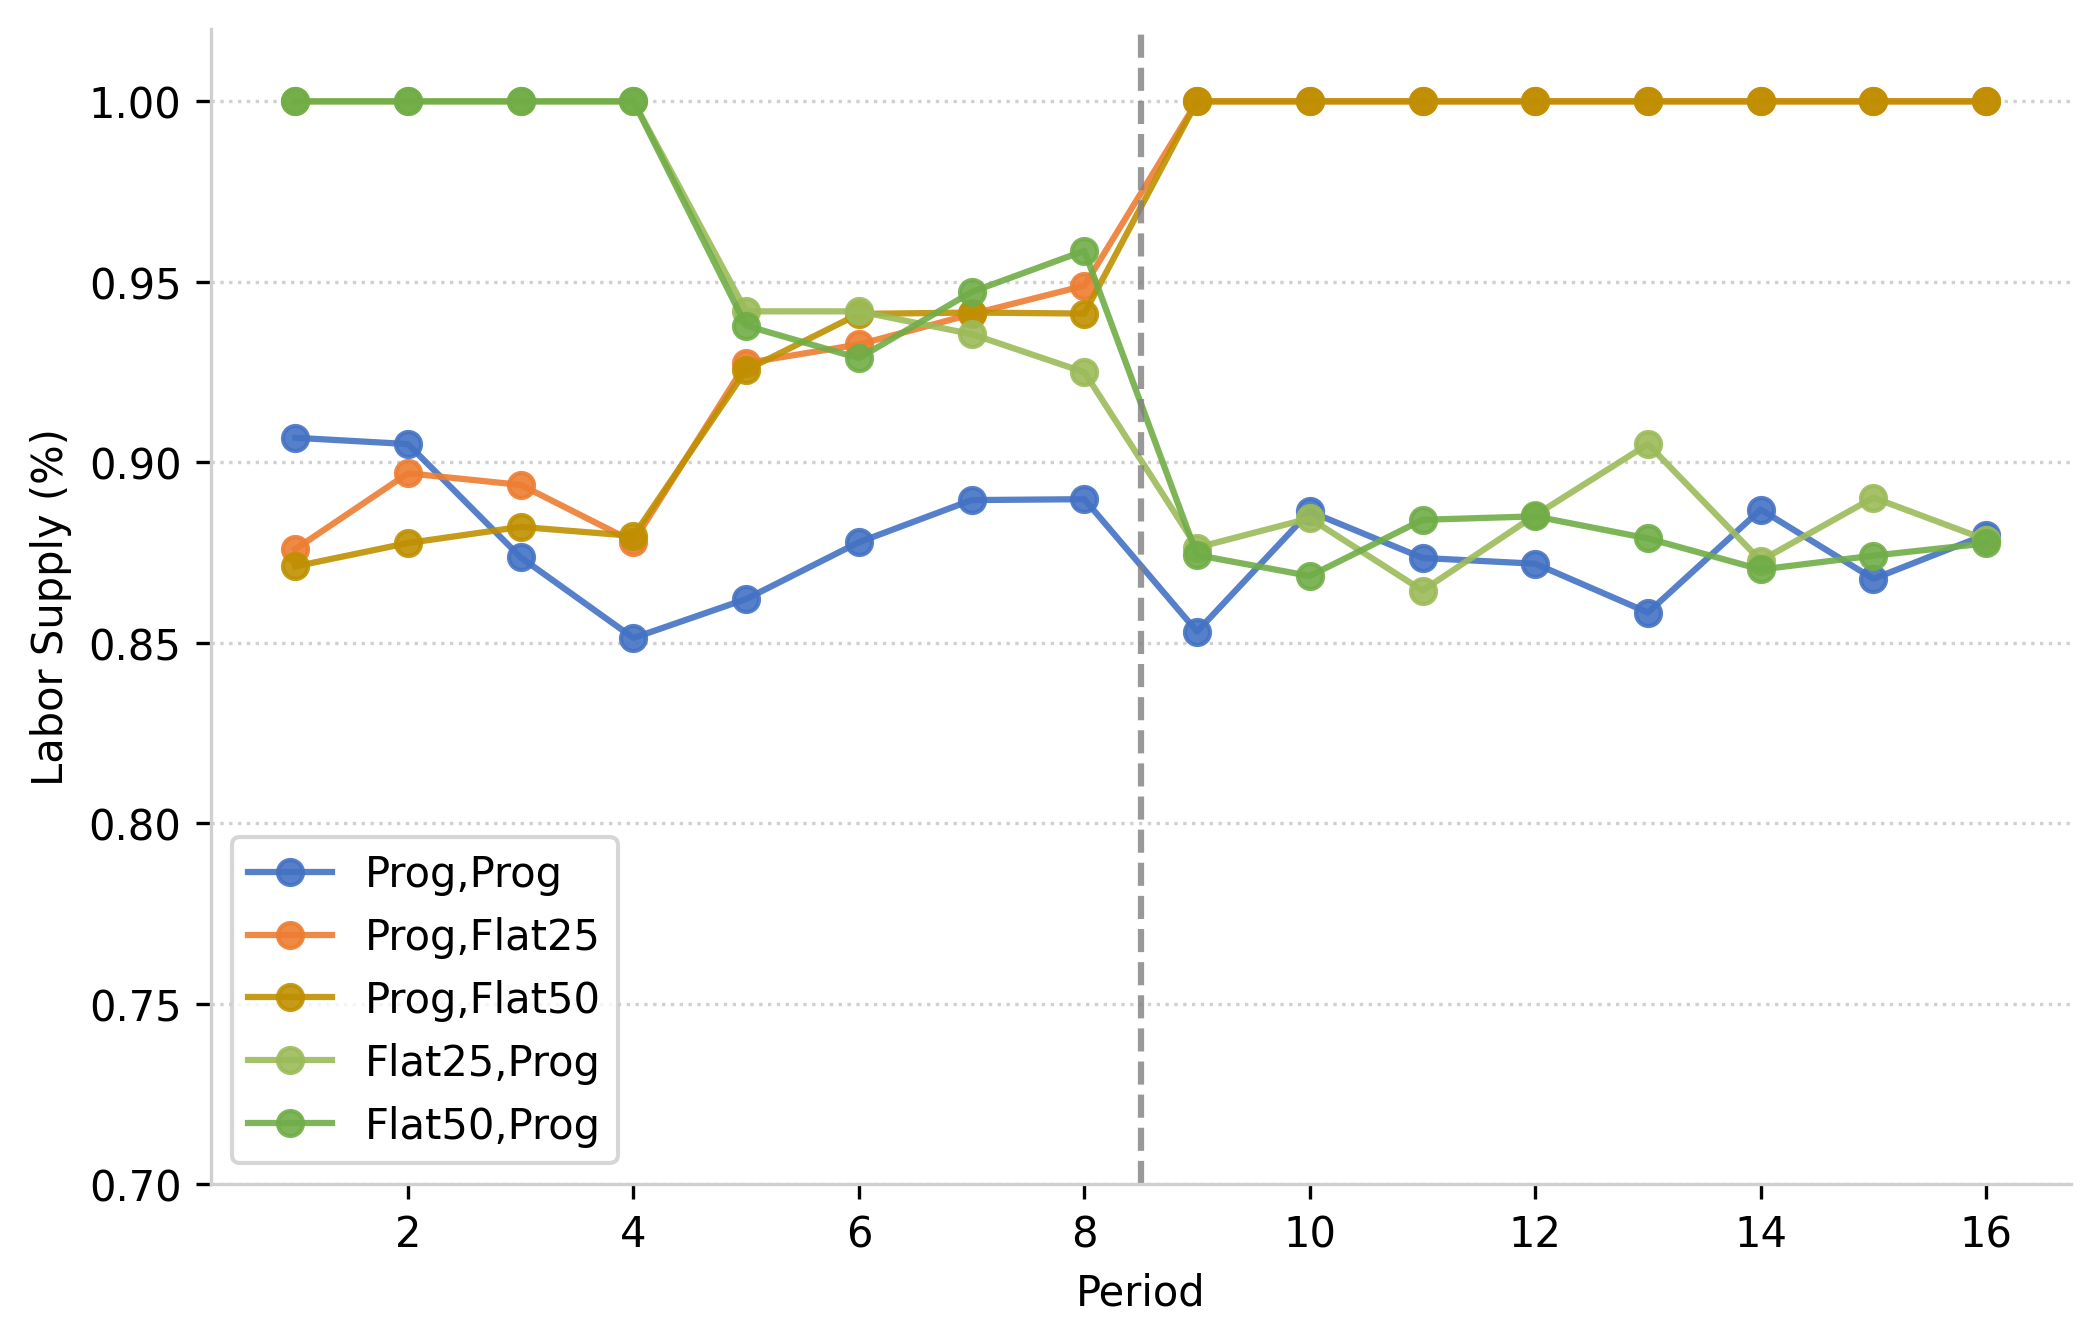
\includegraphics[width=0.47\textwidth]{images_tables/pknf_claude-haiku-4-5-20251001_25pct_50pct_fig4.png}
	}
    \subfigure[DeepSeek V3]{
   	 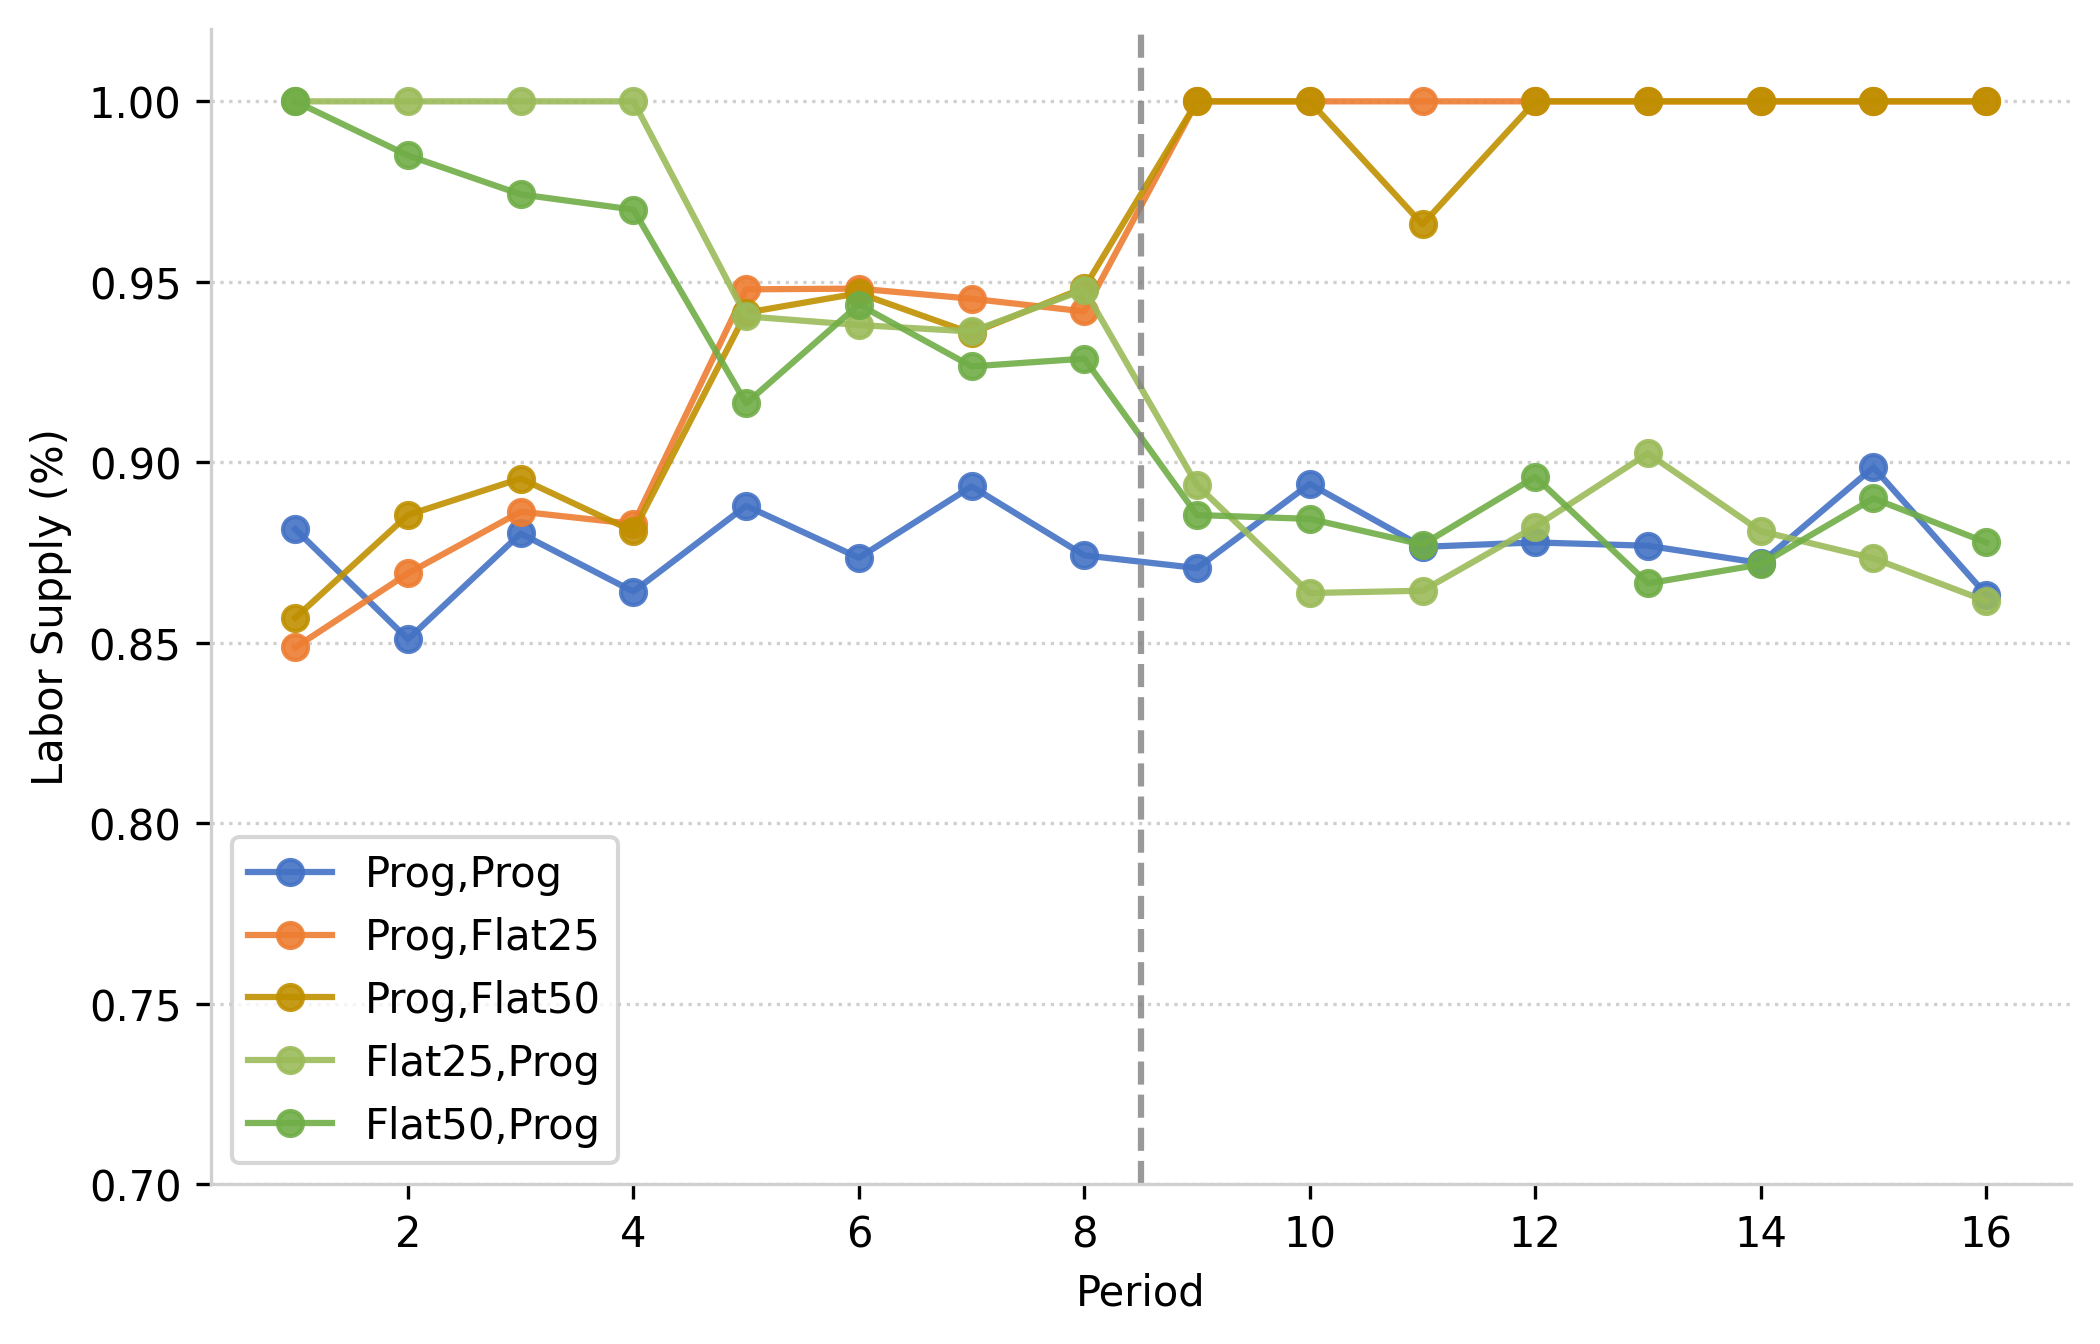
\includegraphics[width=0.47\textwidth]{images_tables/pknf_deepseek-ai_DeepSeek-V3_25pct_50pct_fig4.png}
	}
    \subfigure[Gemma 4]{
   	 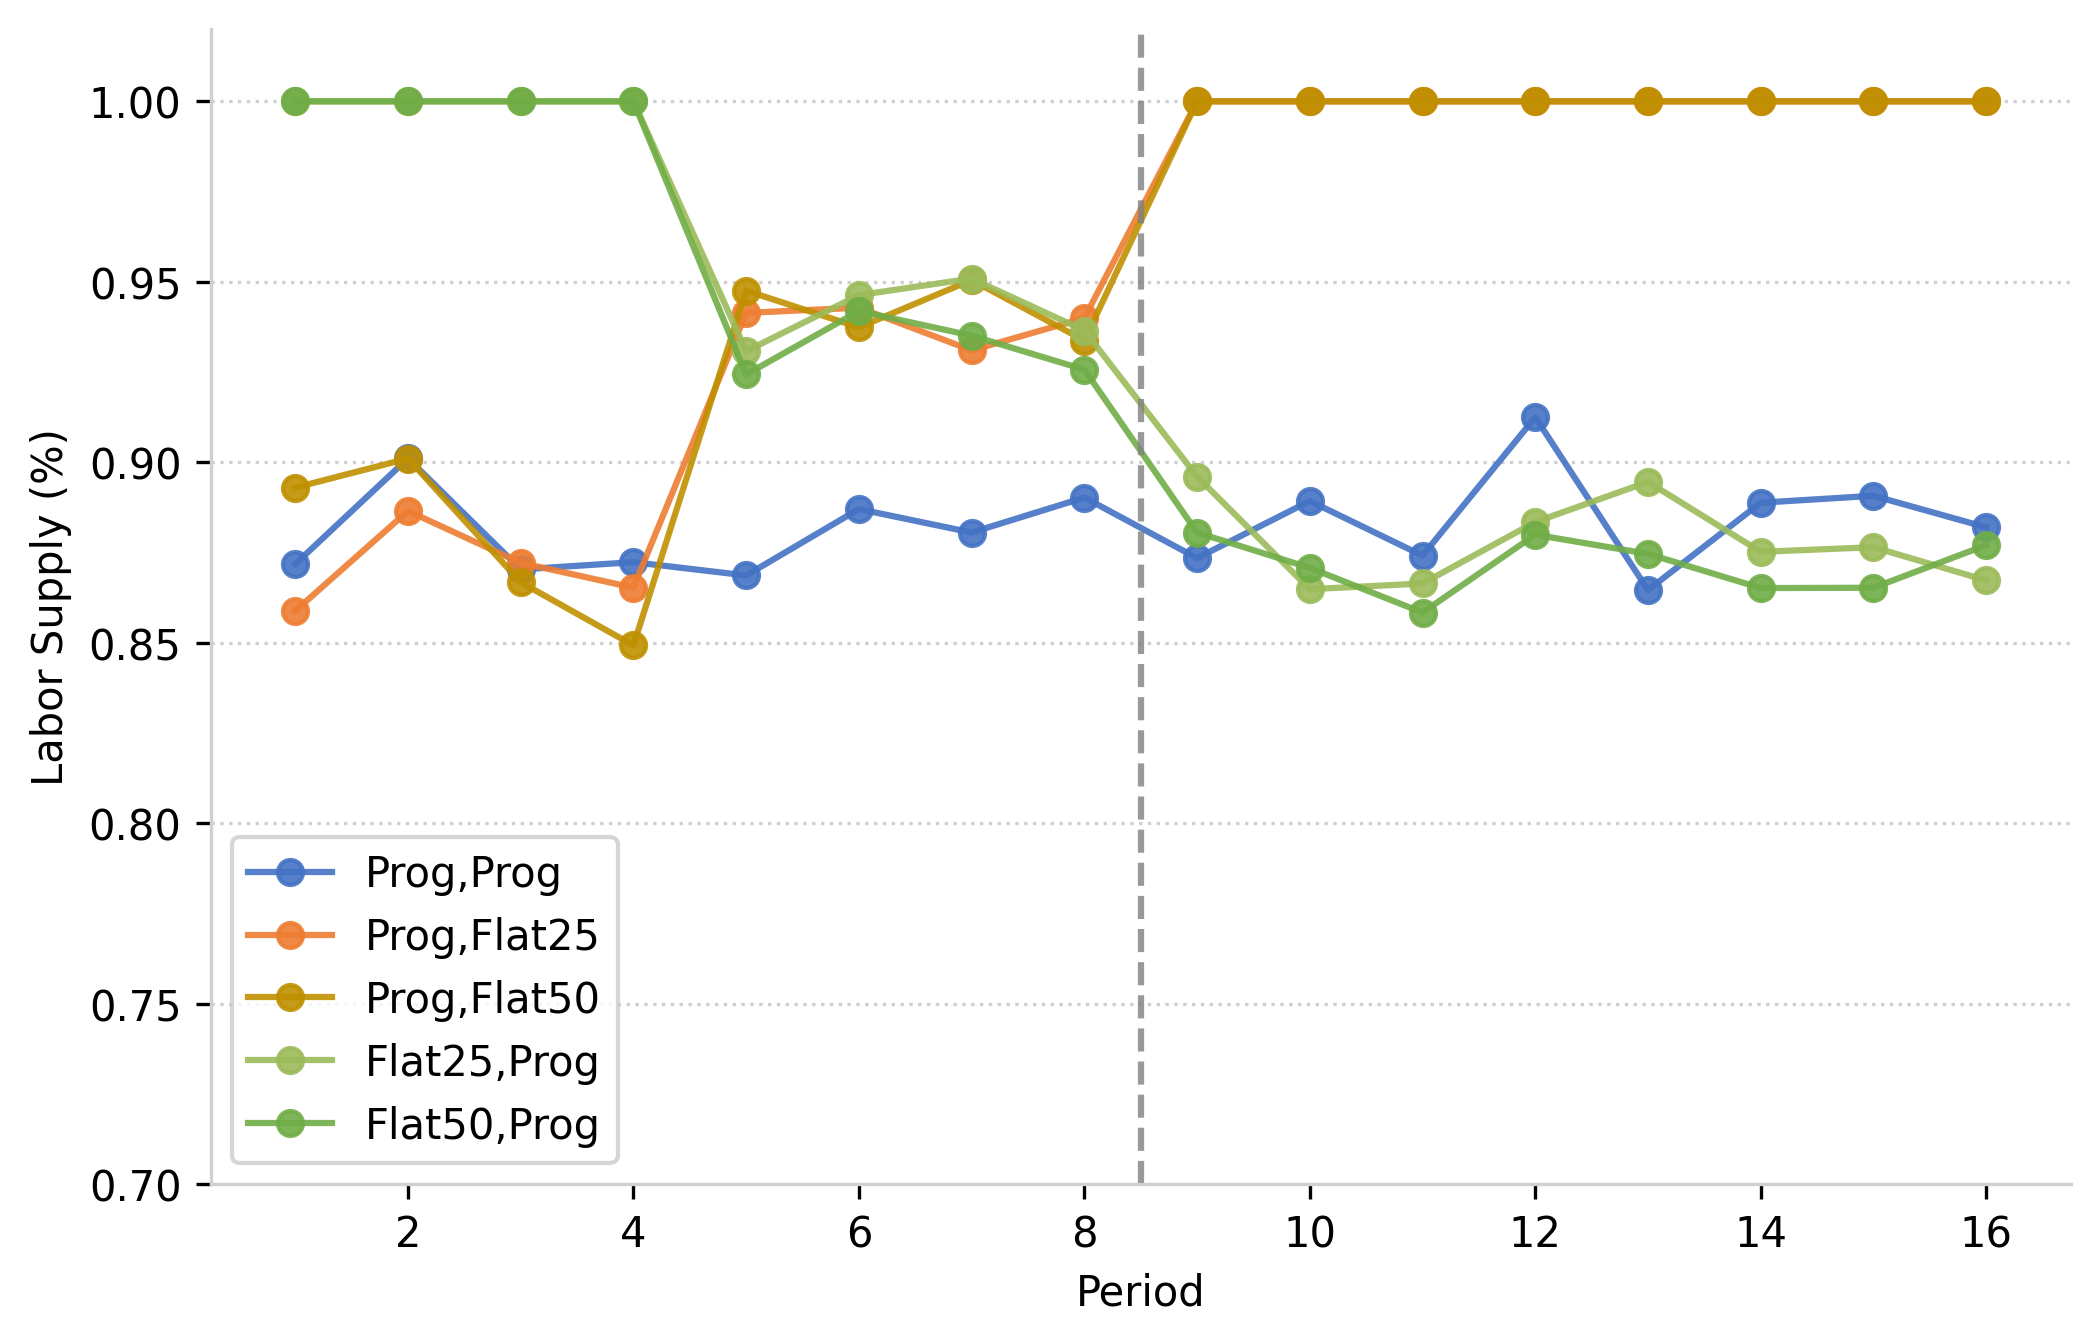
\includegraphics[width=0.47\textwidth]{images_tables/pknf_google_gemma-4-26B-A4B-it_25pct_50pct_fig4.png}
	}
    \small{Figure displays responses by treatment and round for all models.}
    \end{figure}

\newpage
\subsection{Distribution of Pre-Tax Income: All Models}

    \begin{figure}[h]
    \centering
    \caption{Distribution of Pre-Tax Income:} 
    \label{fig:income_dist_all_models}
     \subfigure[GPT-4o-mini]{
   	 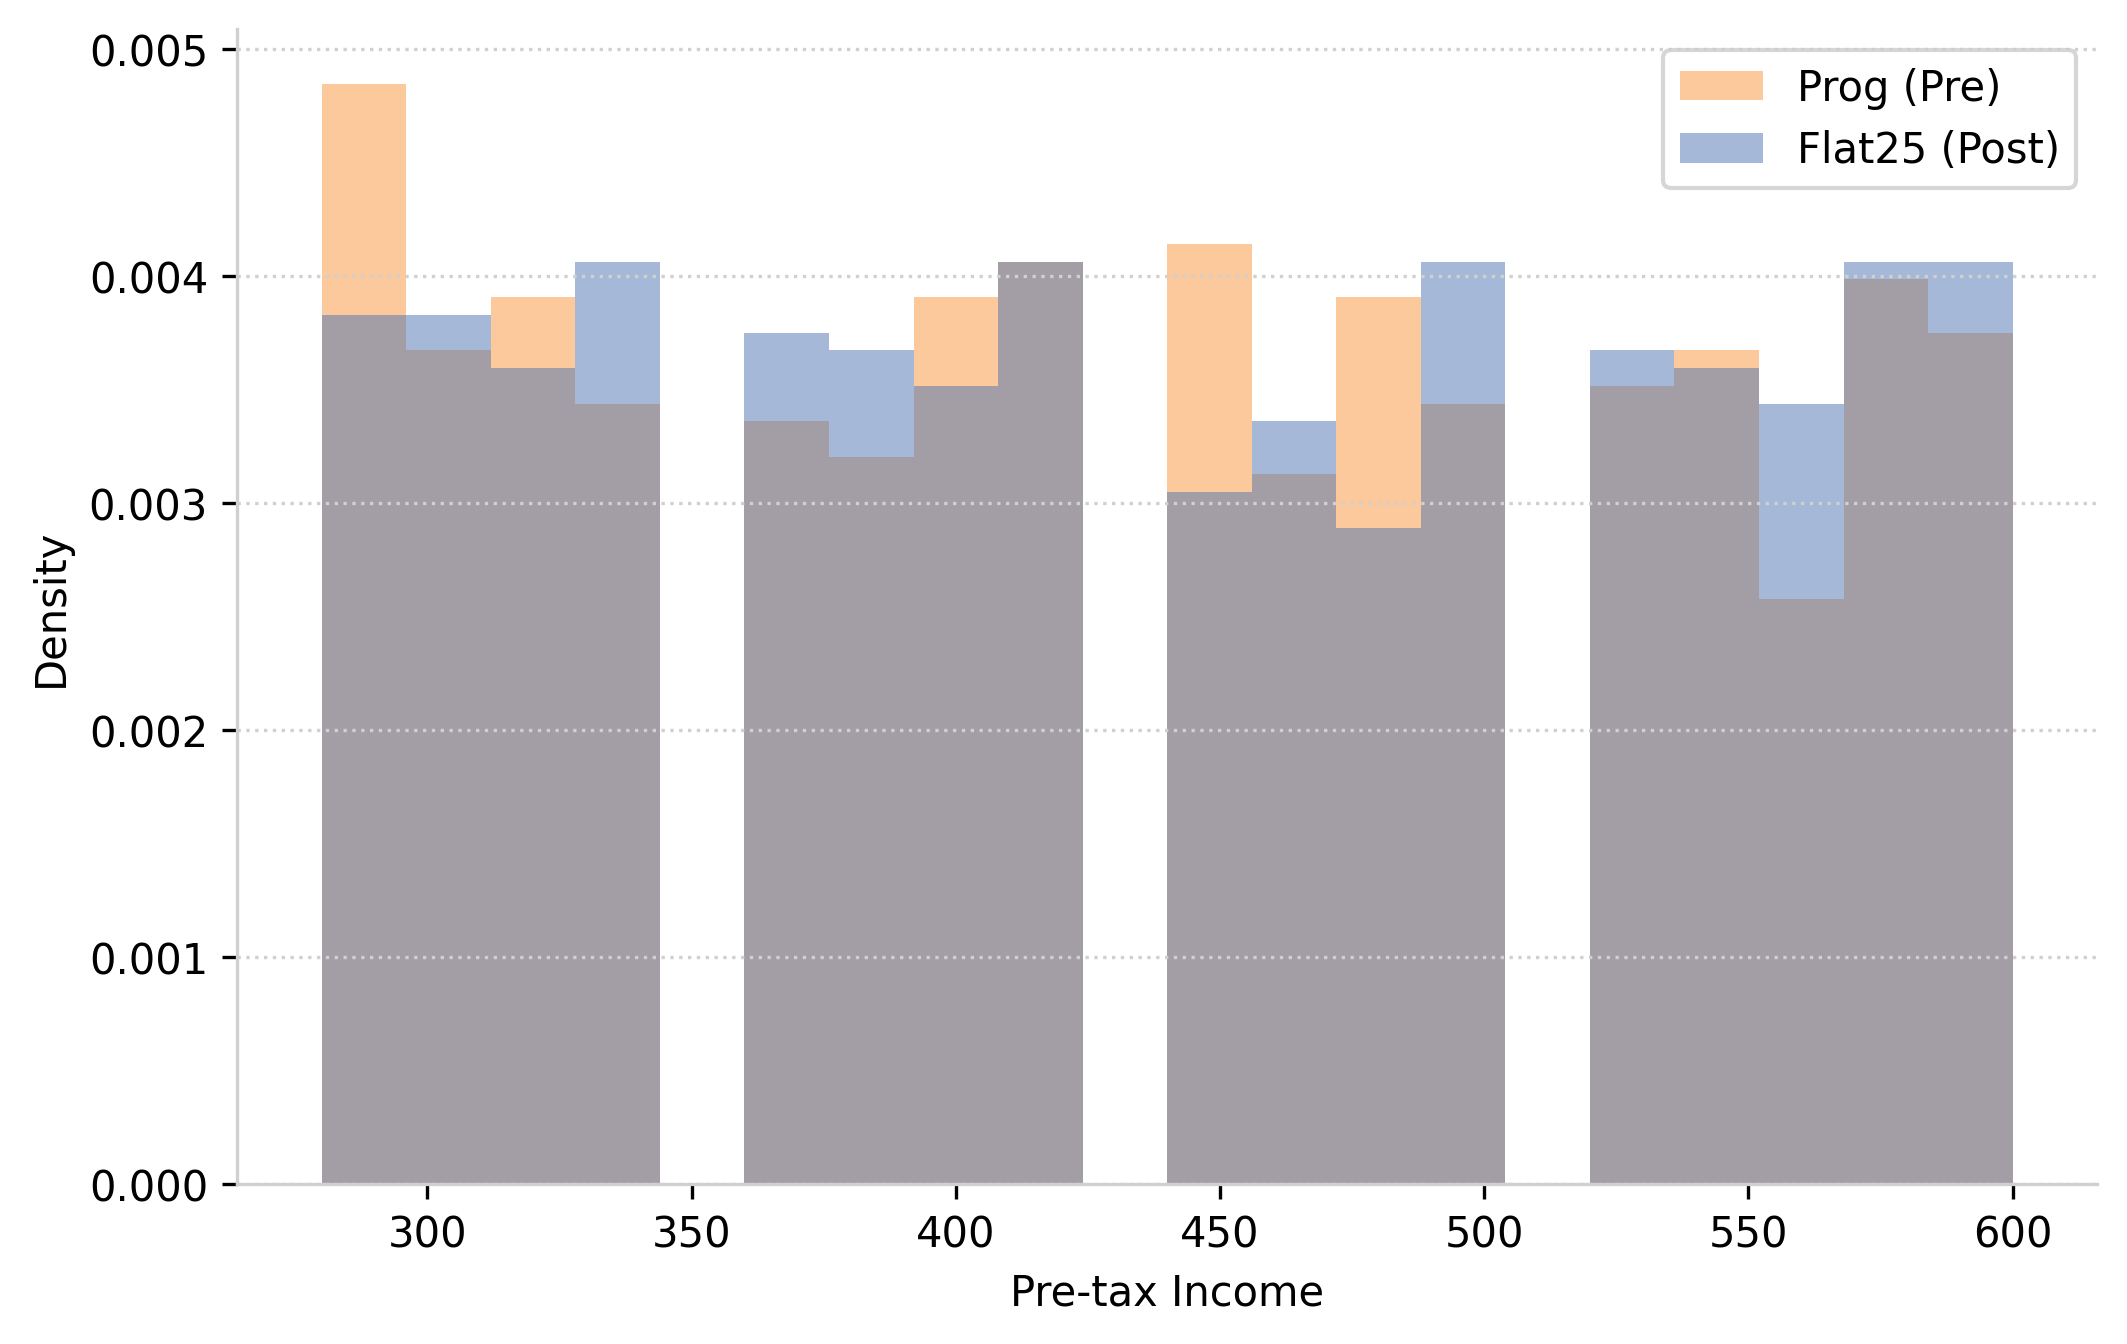
\includegraphics[width=0.47\textwidth]{images_tables/pknf_gpt-4o-mini_25pct_50pct_bunching.png}
	}
    \subfigure[Claude Haiku 4.5]{
   	 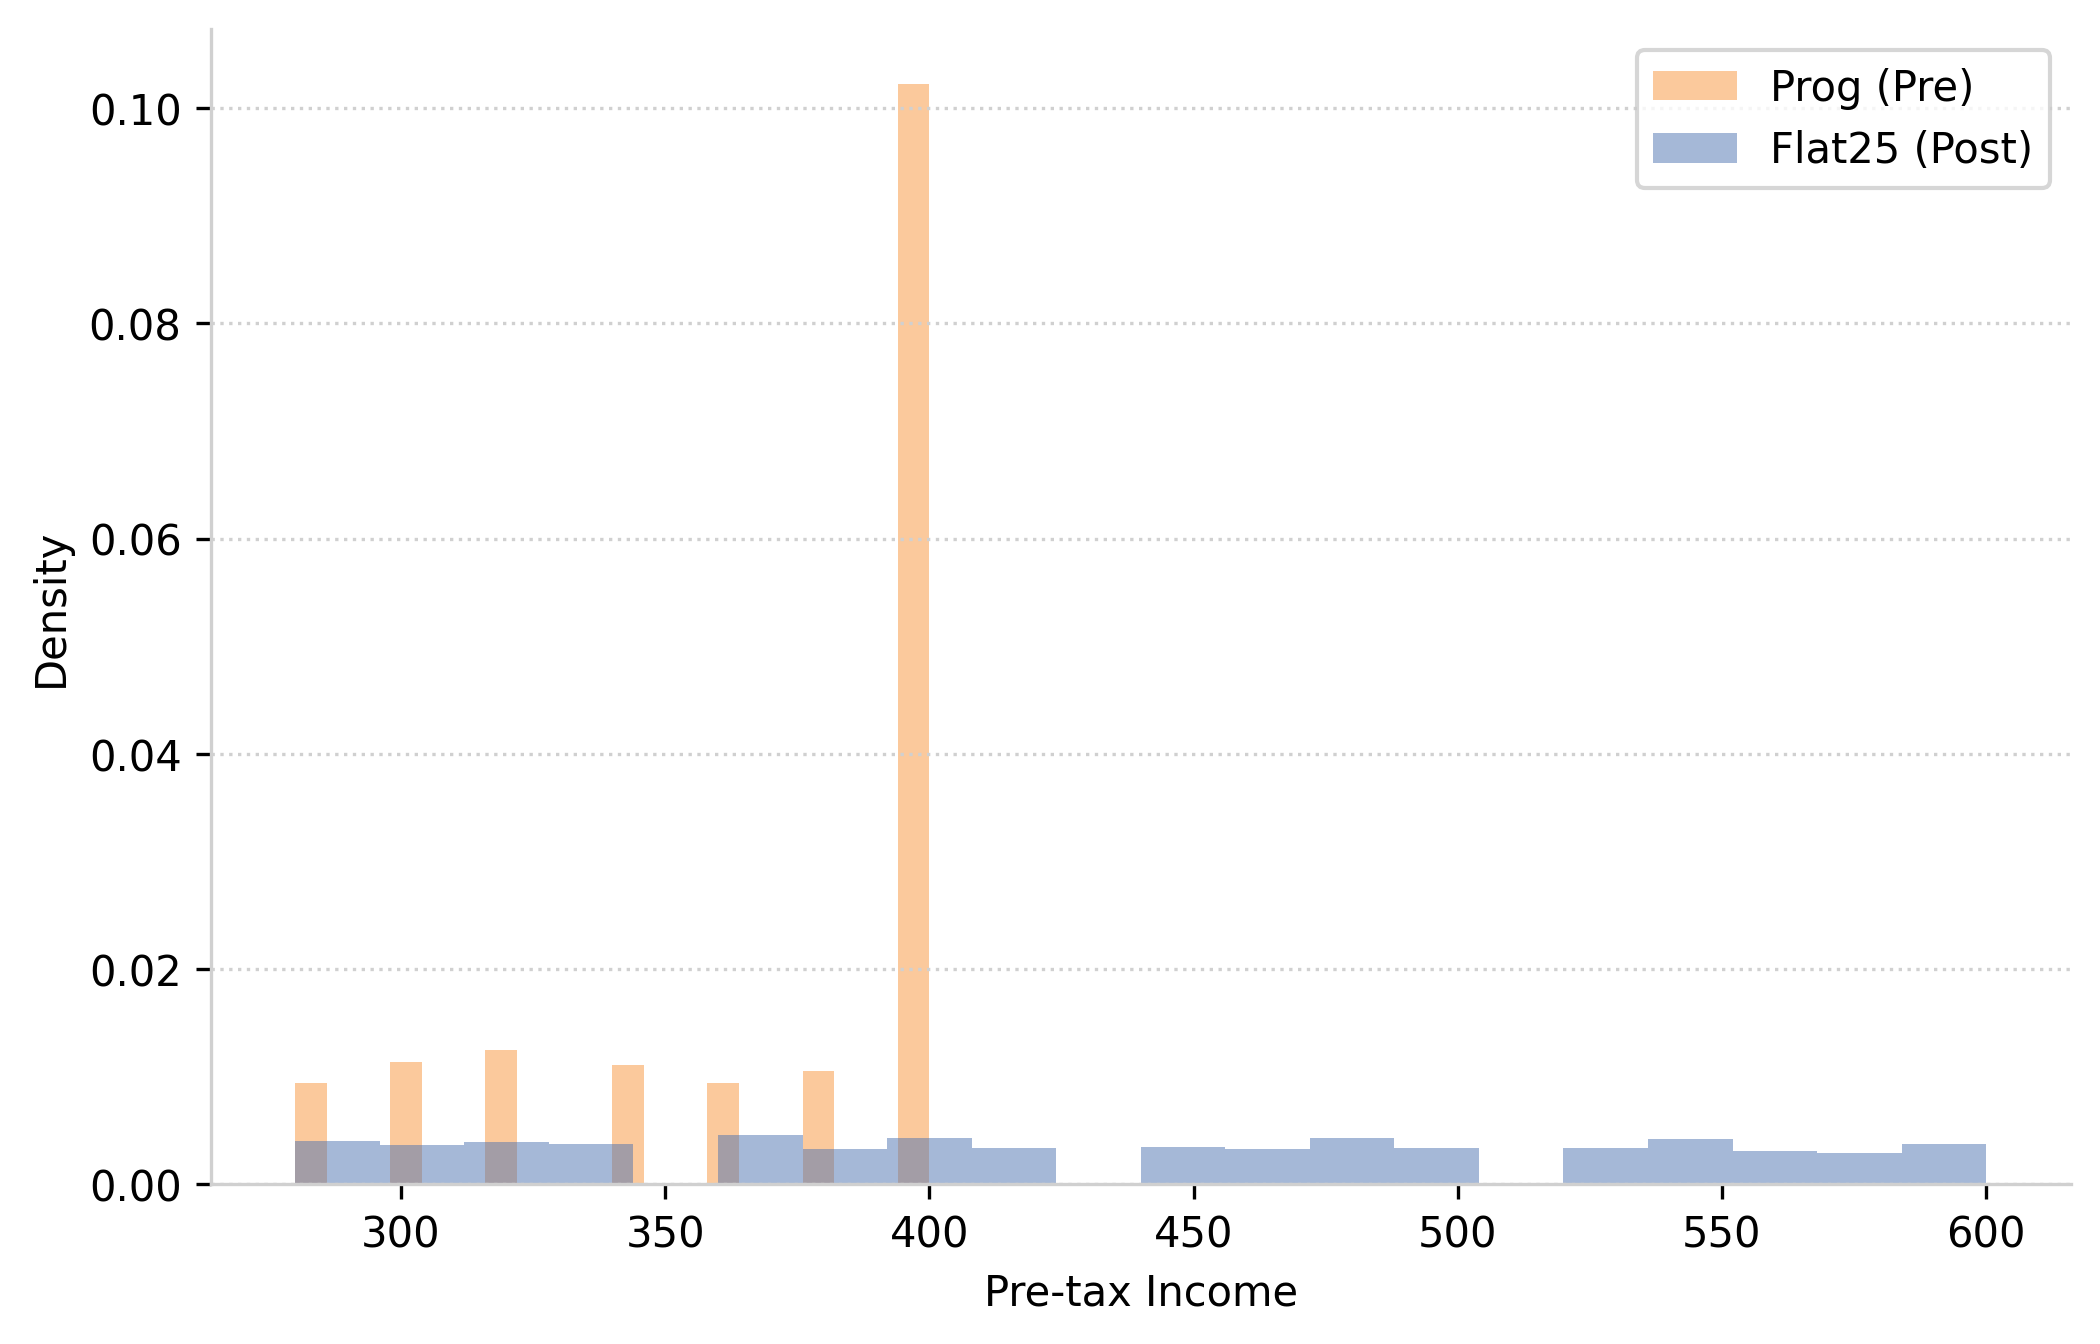
\includegraphics[width=0.47\textwidth]{images_tables/pknf_claude-haiku-4-5-20251001_25pct_50pct_bunching.png}
	}
    \subfigure[DeepSeek V3]{
   	 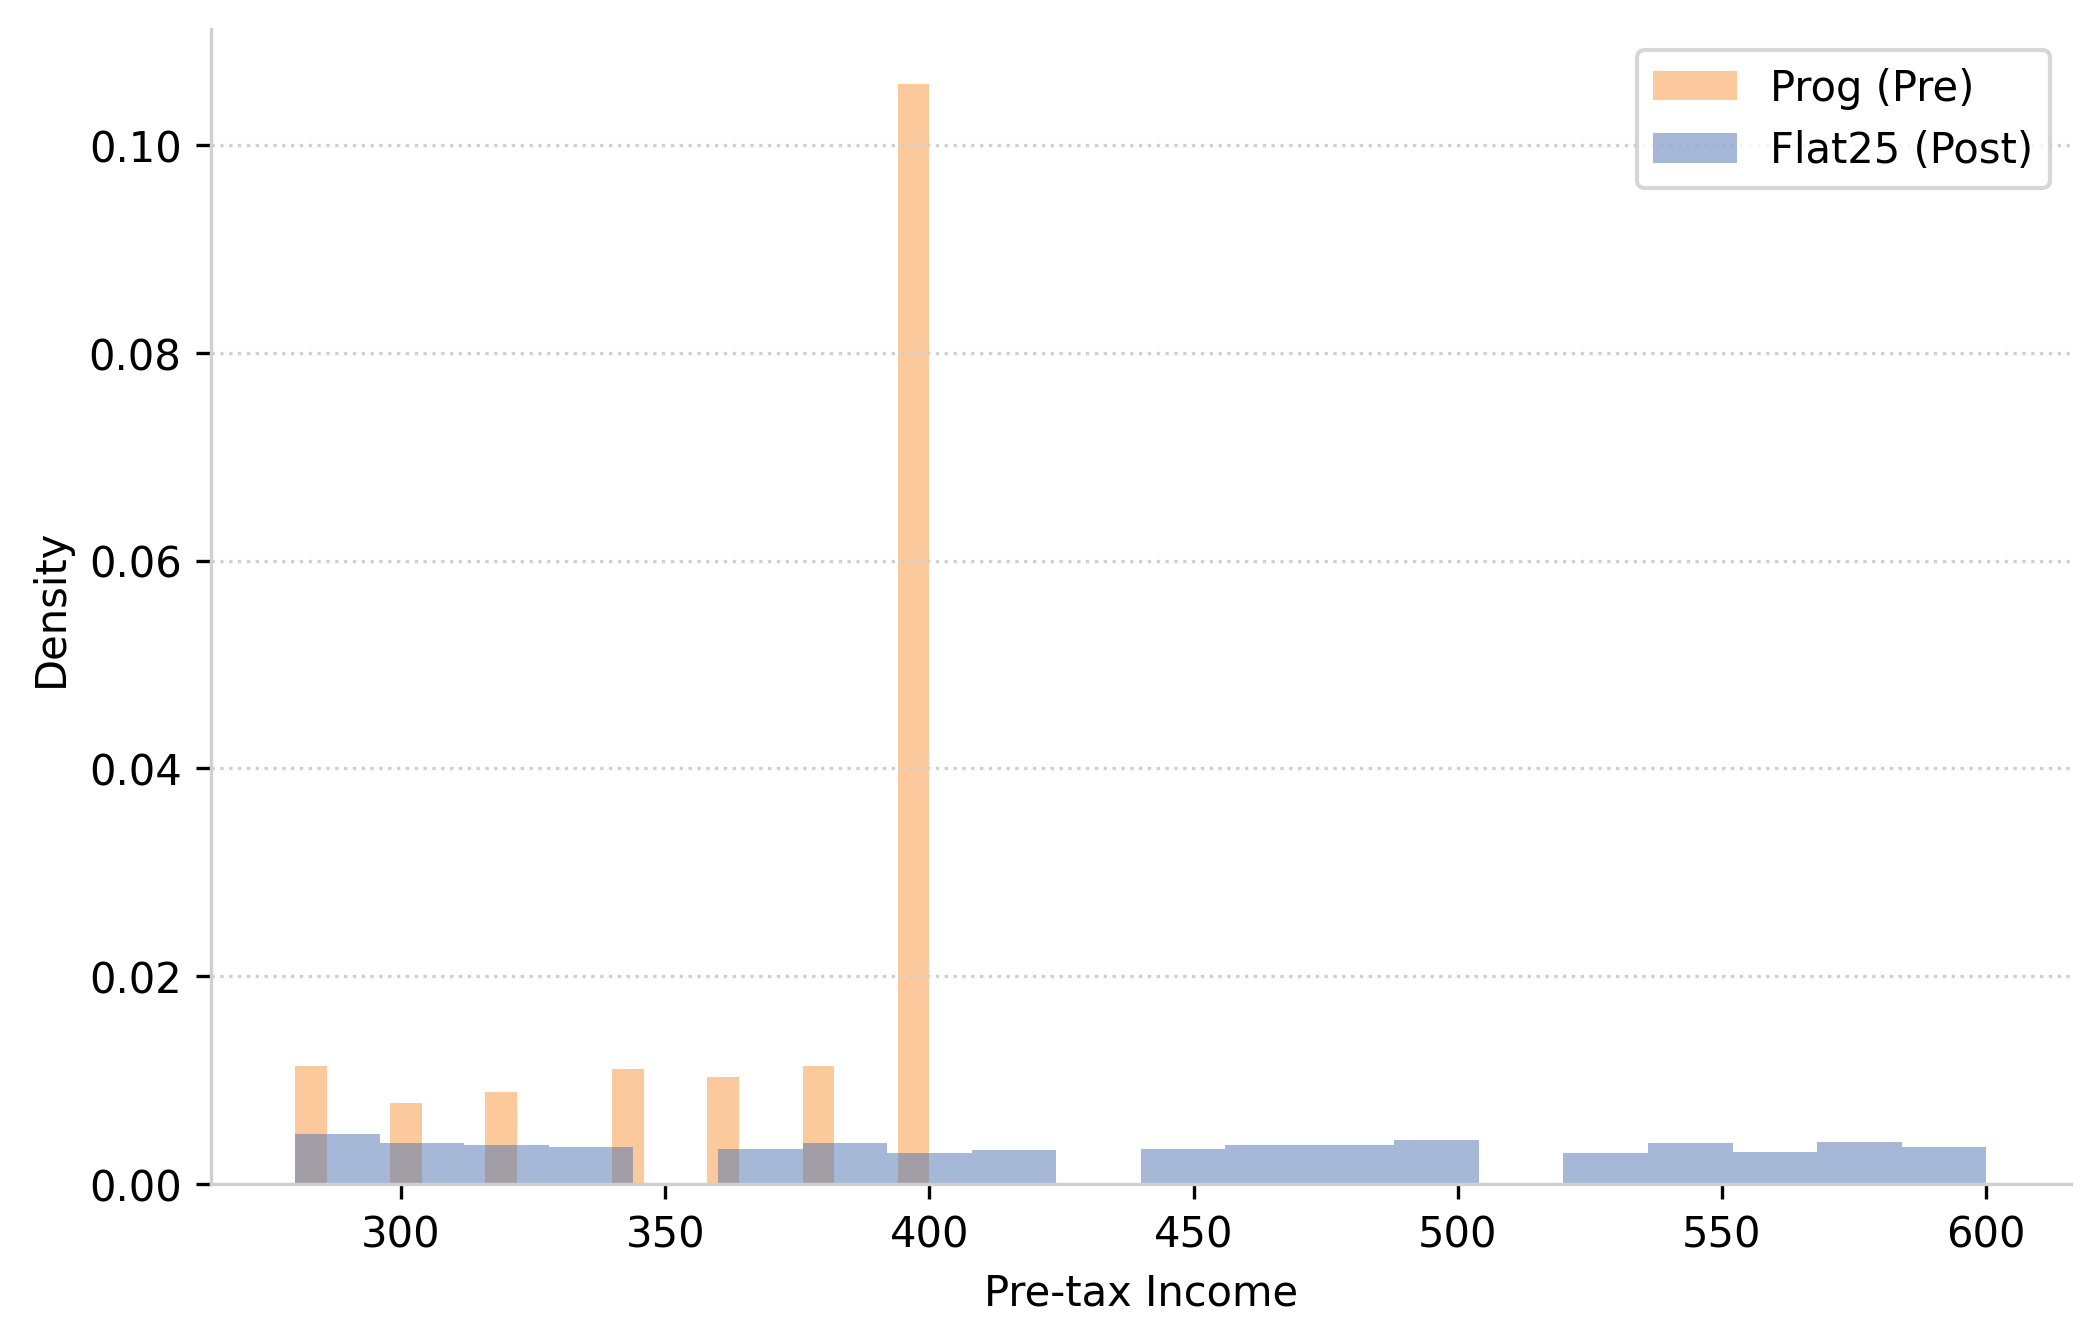
\includegraphics[width=0.47\textwidth]{images_tables/pknf_deepseek-ai_DeepSeek-V3_25pct_50pct_bunching.png}
	}
    \subfigure[Gemma 4]{
   	 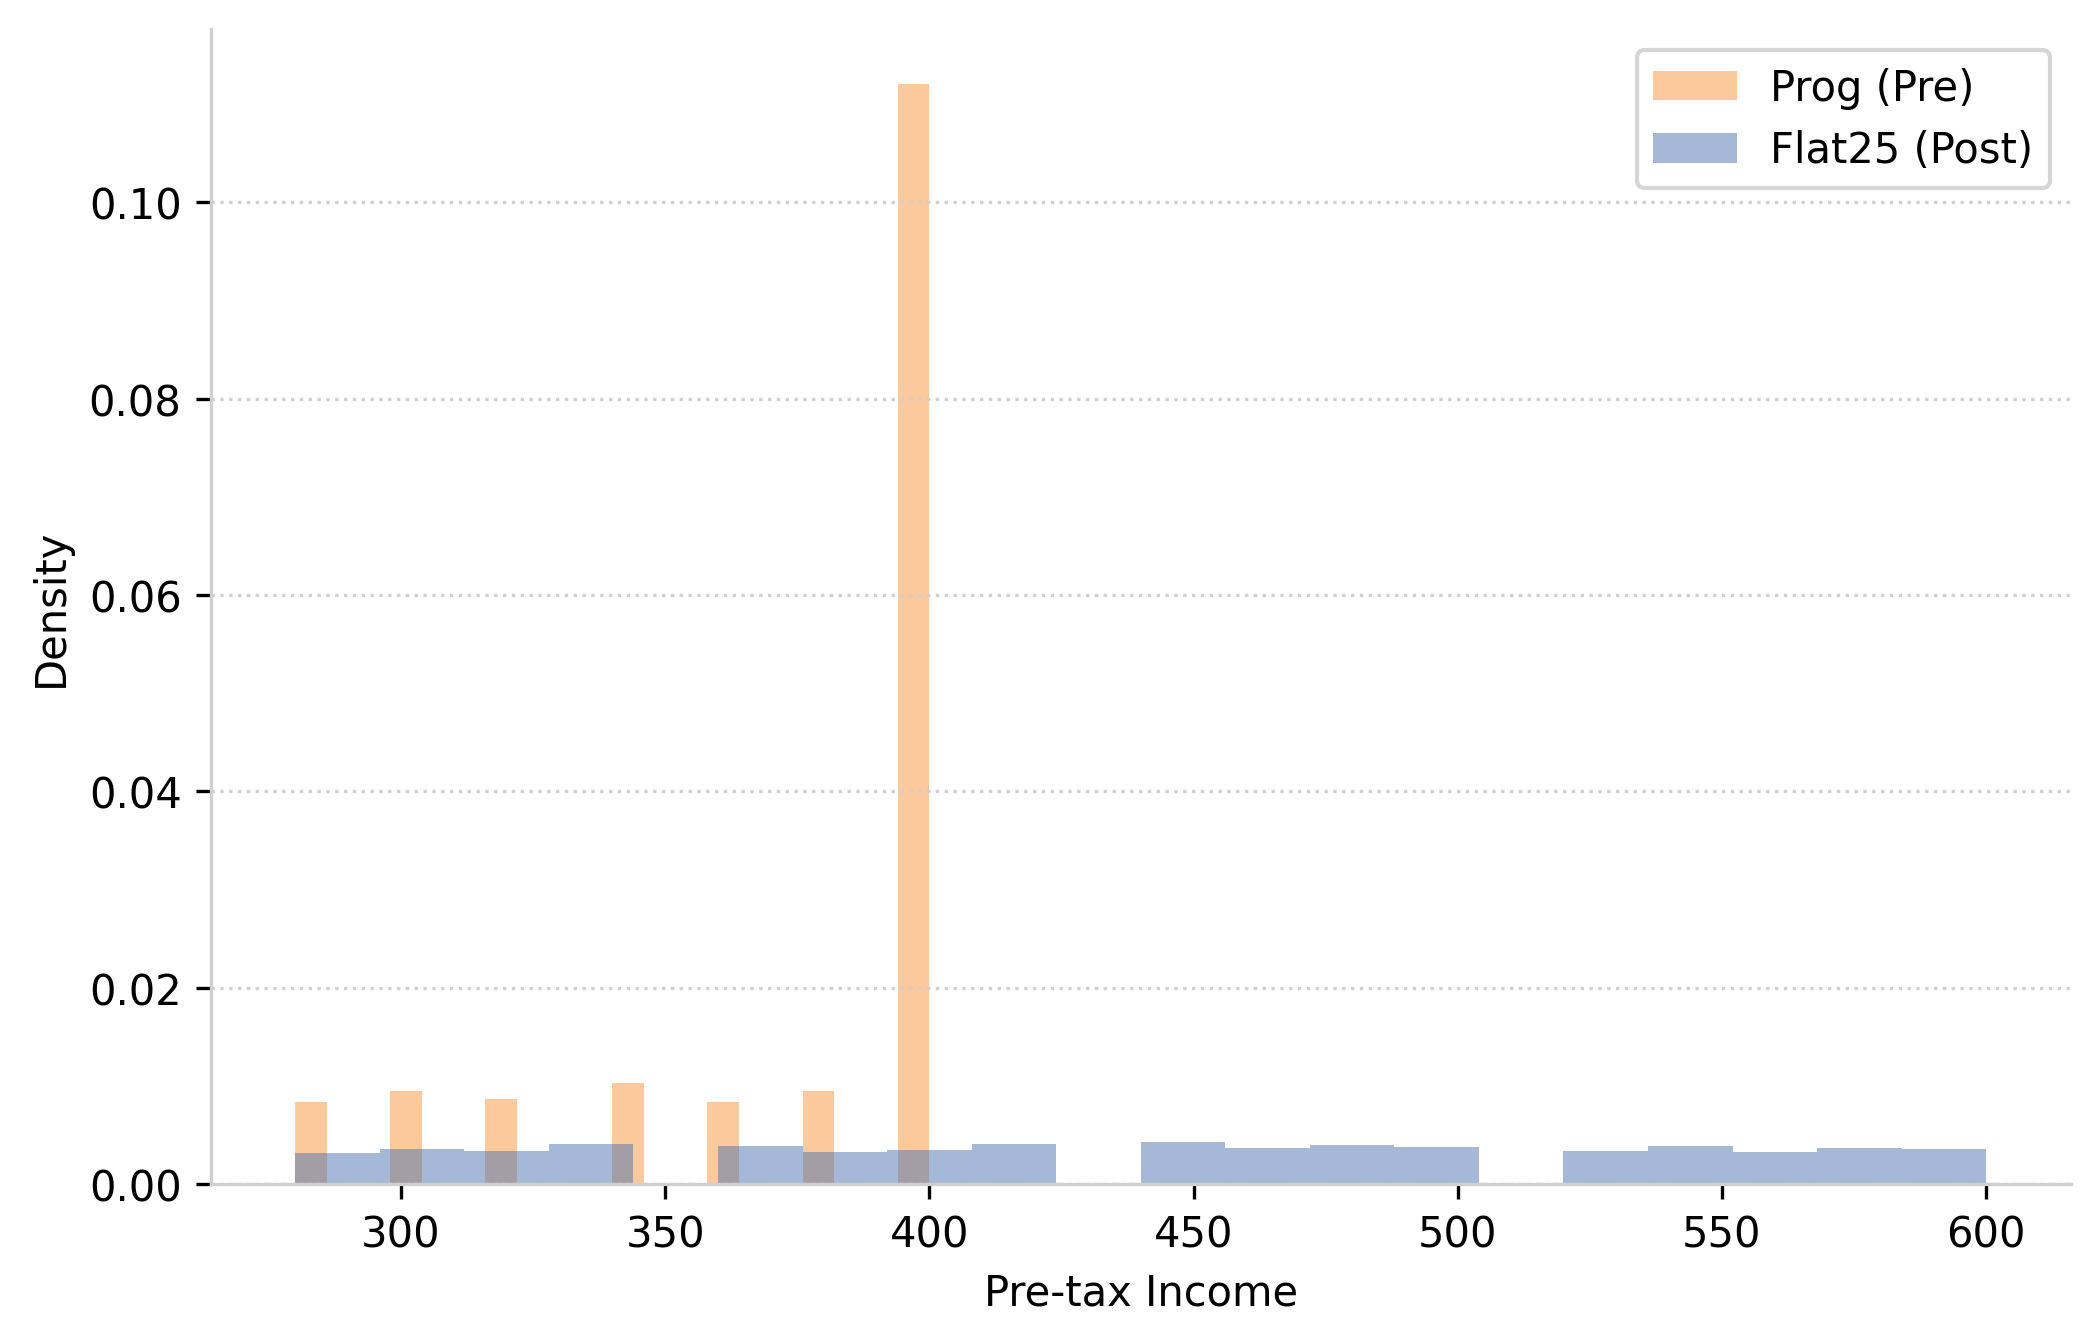
\includegraphics[width=0.47\textwidth]{images_tables/pknf_google_gemma-4-26B-A4B-it_25pct_50pct_bunching.png}
	}
    \small{Figure displays the distributions of pre-tax income.}
    \end{figure}

\newpage
\subsection{Distribution of Pre-Tax Income: Alternative Parameterization (40\% Top Rate): All Models}

    \begin{figure}[h]
    \centering
    \caption{Distribution of Pre-Tax Income: Alternative Parameterization (40\% Top Rate)} 
    \label{fig:income_dist_all_models_alt}
     \subfigure[GPT-4o-mini]{
   	 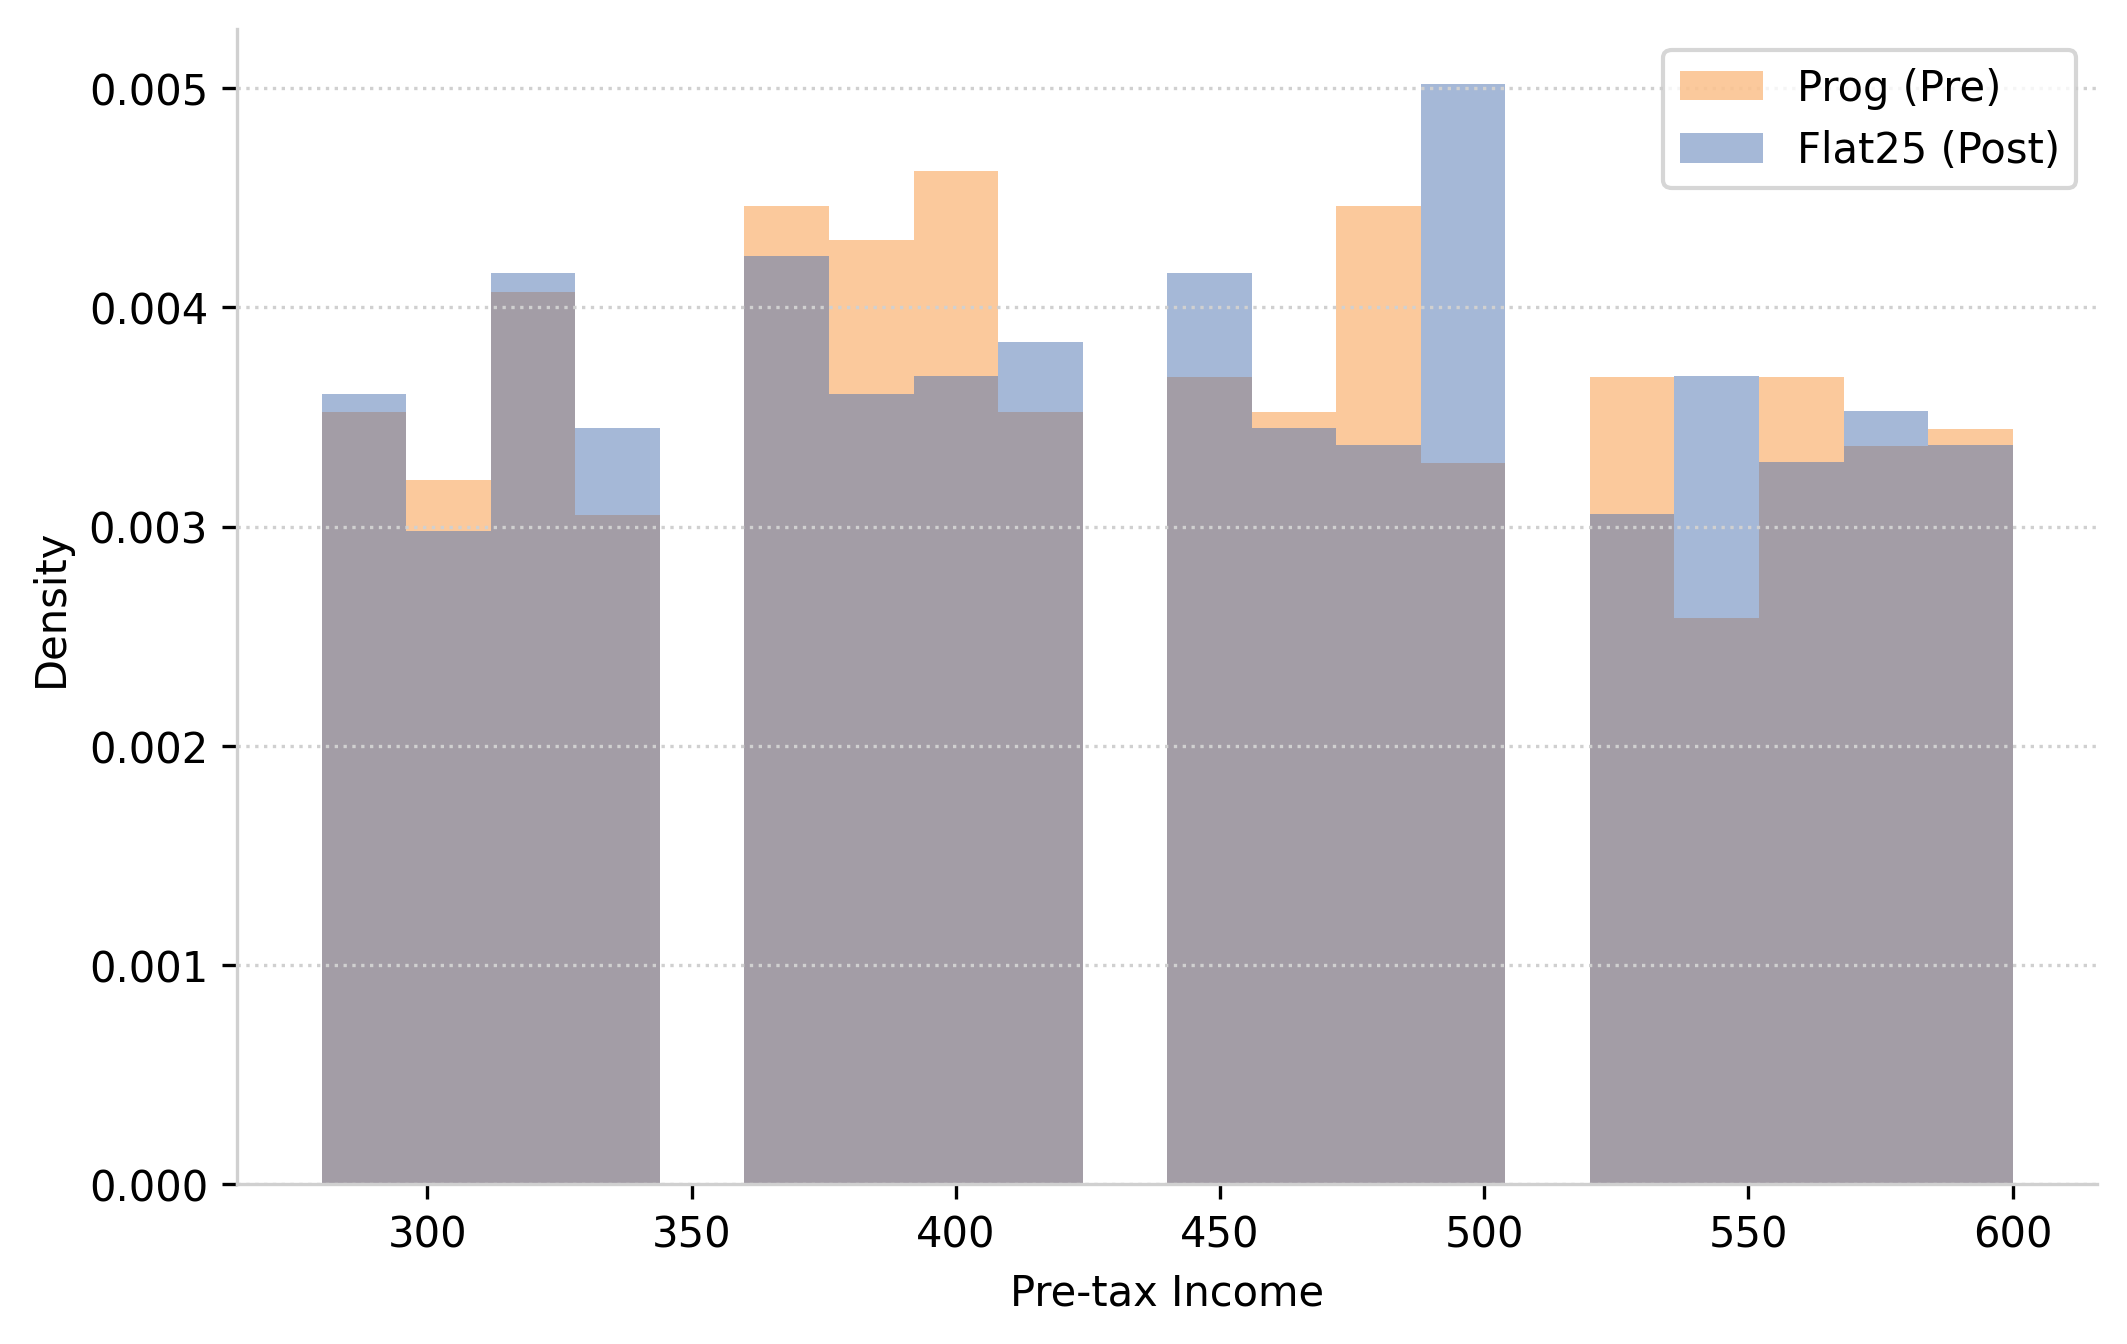
\includegraphics[width=0.47\textwidth]{images_tables/pknf_gpt-4o-mini_25pct_40pct_bunching.png}
	}
    \subfigure[Claude Haiku 4.5]{
   	 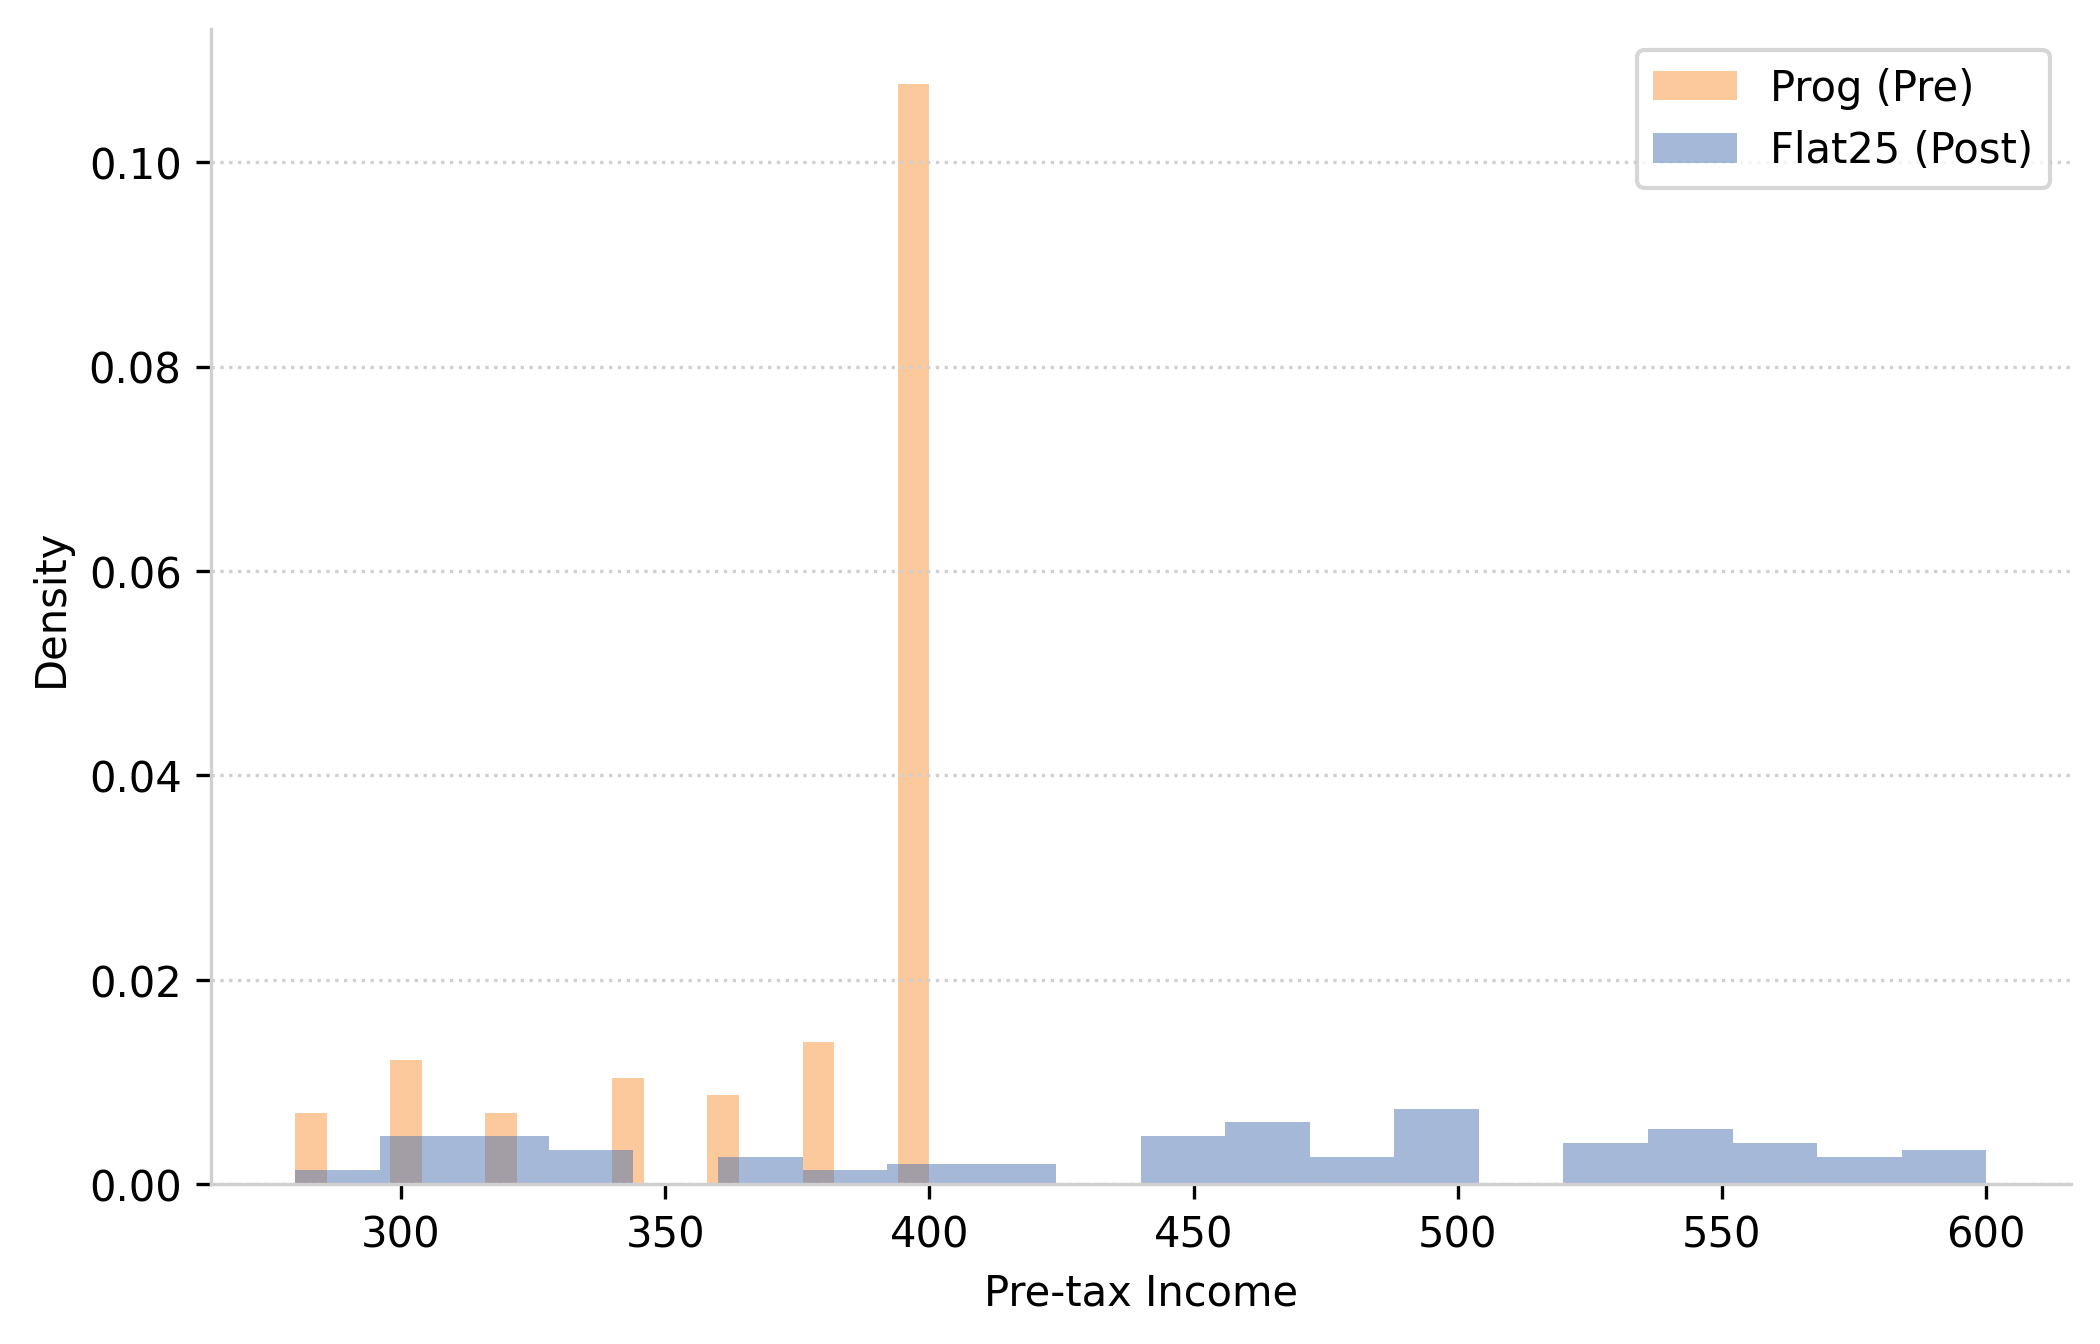
\includegraphics[width=0.47\textwidth]{images_tables/pknf_claude-haiku-4-5-20251001_25pct_40pct_bunching.png}
	}
    \subfigure[DeepSeek V3]{
   	 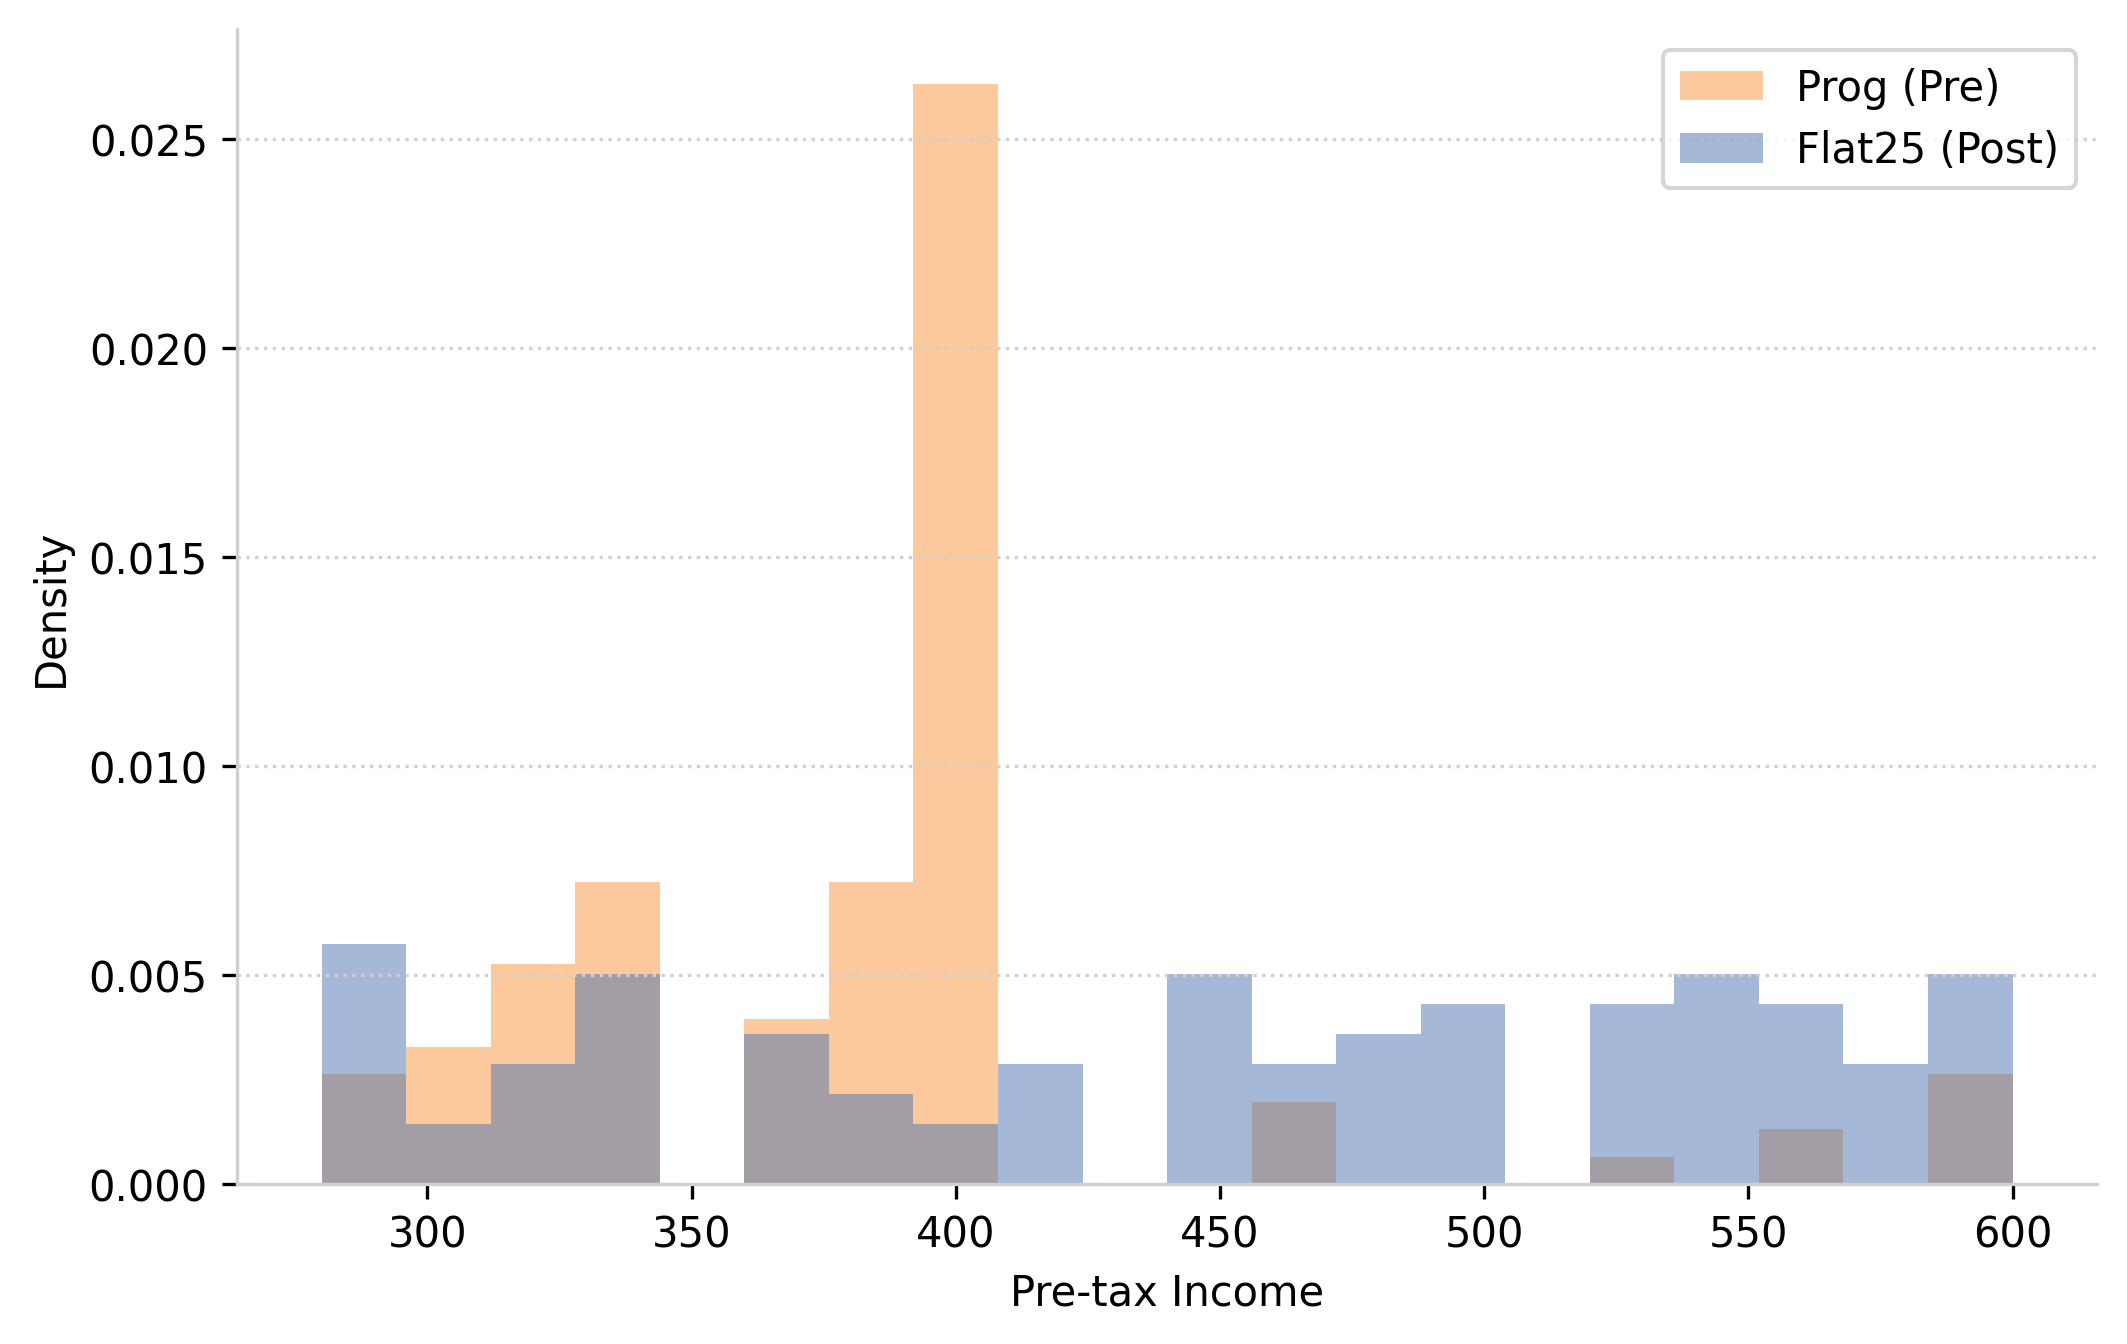
\includegraphics[width=0.47\textwidth]{images_tables/pknf_deepseek-ai_DeepSeek-V3_25pct_40pct_bunching.png}
	}
    \subfigure[Gemma 4]{
   	 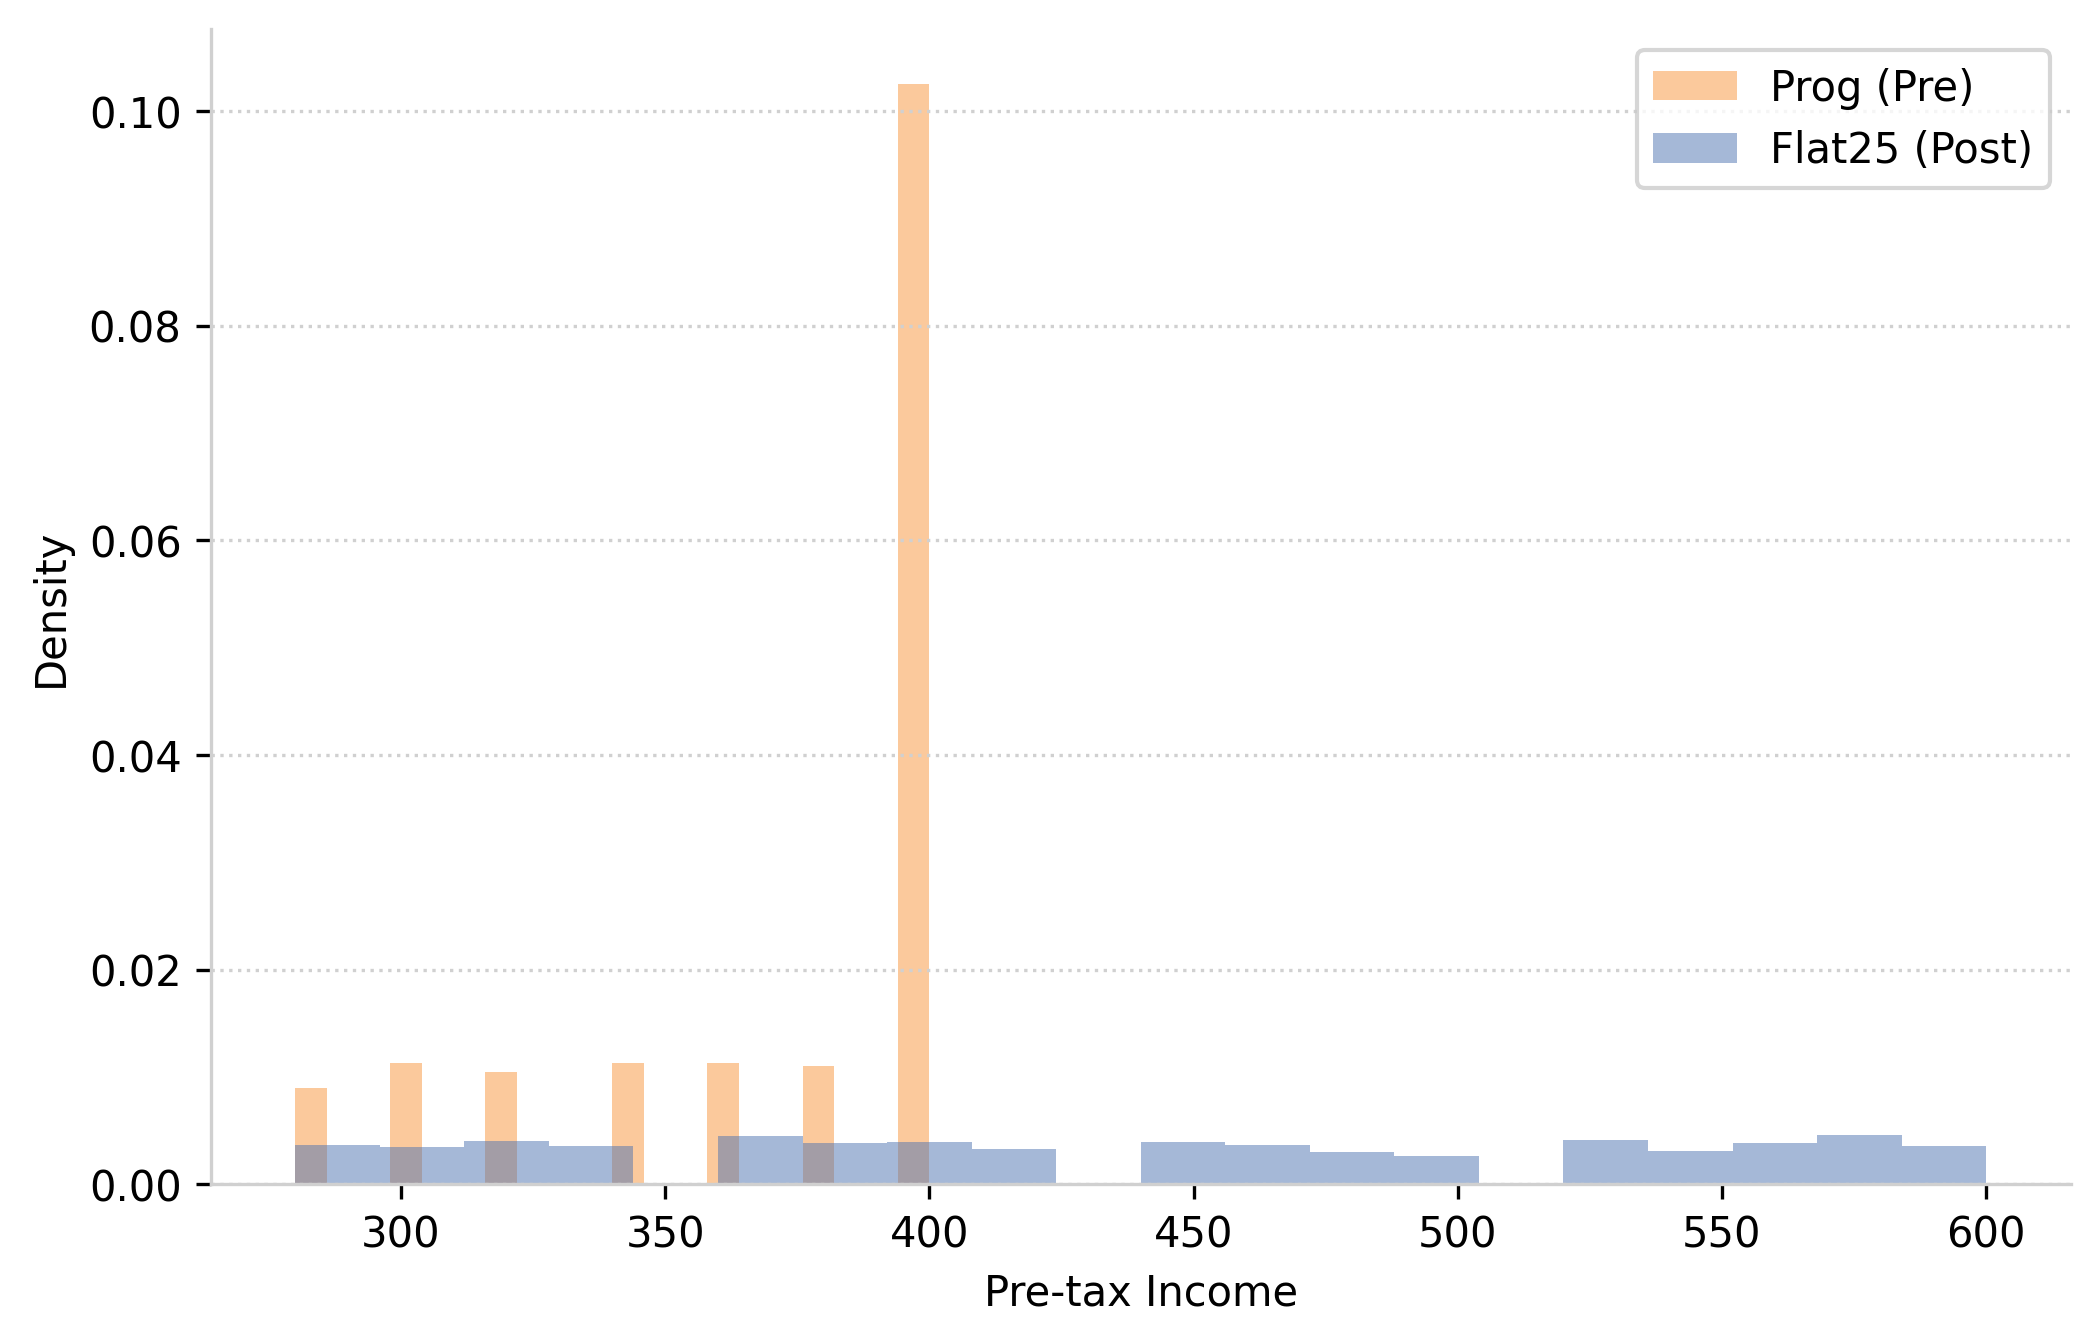
\includegraphics[width=0.47\textwidth]{images_tables/pknf_google_gemma-4-26B-A4B-it_25pct_40pct_bunching.png}
	}
    \small{Figure displays the distributions of pre-tax income.}
    \end{figure}

\end{spacing}


\end{document}
